% =============================================================
% Master's Thesis — Institut Teknologi Bandung, Smart System
% =============================================================
% STATUS: revised draft manuscript, not a final/defensible thesis.
% Distinct from docs/proposal-latex/ (the research PROPOSAL
% skeleton) — do not confuse the two. See README.md for status,
% and FORMAT_COMPLIANCE.md for the page-by-page mapping of this
% preamble's formatting choices to the supplied ITB guide
% (fc0779-juknis_tesis_Mei2019_rev.pdf, "Petunjuk Teknis Penulisan
% Tesis Magister," ITB Sekolah Pascasarjana, Juni 2017) and the
% matching template-tesis_Mei2019.docx.
%
% TEMPLATE STATUS: no official ITB/program-specific .cls or .sty
% file was found anywhere in this repository (searched for *.cls,
% *.sty, *itb*, *smart-system*). itb-thesis.sty (this directory)
% is an UNOFFICIAL formatting layer derived directly from the two
% supplied sources above — see that file's header comment and
% FORMAT_COMPLIANCE.md for exactly which rule came from which
% source, and the compile-verified status of each rule (see
% README.md "Compilation Status").
%
% THIS FILE IS DELIBERATELY THIN. It is the compiled entry point
% (TeX requires one file with \documentclass + \begin{document}),
% but everything that changes day-to-day lives elsewhere:
%   - config.tex      — title, author, NIM, supervisors, dates.
%                        Edit THIS, not main.tex, to fill in your
%                        own thesis's metadata.
%   - itb-thesis.sty   — margins, fonts, heading/numbering rules.
%                        Edit THIS to change formatting.
%   - structure.tex    — the actual document body: frontmatter and
%                        chapter \input order. Edit THIS to add,
%                        remove, or reorder chapters/frontmatter
%                        pages — not main.tex.
% See README.md "Project Layout" for the full file map.
% =============================================================

\documentclass[12pt,a4paper]{report}
\usepackage{itb-thesis}

% =============================================================
% config.tex — Single source of truth for thesis metadata
% =============================================================
% Thesis metadata only. Update this file when the official title,
% author details, supervisors, and approval date are confirmed.
% =============================================================

% --- Thesis identity ------------------------------------------

% Proposed working title; pending supervisor approval.
\newcommand{\ThesisTitleID}{Evaluasi Kesenjangan Kinerja Pengenalan Ekspresi Wajah antar-Kelompok Kecerahan Kulit pada Potongan Wajah dari Film Dokumenter Papua: HSEmotion, CLAHE, dan ArcFace dengan Regresi Logistik}

\newcommand{\ThesisTitleEN}{Evaluating Facial Expression Recognition Performance Gaps between Skin-Brightness Groups on Face Crops from a Papuan Documentary Film: HSEmotion, CLAHE, and ArcFace with Logistic Regression}

% Plain-text companions for PDF metadata.
% Keep these synchronized with the official thesis title.
\newcommand{\ThesisTitlePlain}{Evaluasi Kesenjangan Kinerja Pengenalan Ekspresi Wajah antar-Kelompok Kecerahan Kulit}

\newcommand{\ThesisAuthorPlain}{Marde Fasma'ul Aza}

% --- Author ----------------------------------------------------

\newcommand{\ThesisAuthor}{Marde Fasma'ul Aza}
\newcommand{\ThesisNIM}{23524301}
\newcommand{\ThesisProgramID}{Program Studi Magister Smart System}
\newcommand{\ThesisProgramEN}{Master's Program in Smart System}

% --- Institution / date ---------------------------------------

\newcommand{\ThesisInstitution}{Institut Teknologi Bandung}
\newcommand{\ThesisMonthYear}{Oktober 2026}
\newcommand{\ThesisApprovalDate}{\TODO{Tanggal Pengesahan}}

% --- Supervisor (Pembimbing) -----------------------------------
% Single supervisor, matching the reference thesis
% "23524315_Yogi Putra_PT Pos.pdf" (same pembimbing, confirmed by
% the user), whose Lembar Pengesahan lists exactly one name under
% "Pembimbing" (no separate Ketua/Anggota committee):
%   Dr. Fadhil Hidayat, S.Kom., M.T.
% frontmatter/pengesahan.tex was simplified to match this
% single-supervisor layout; see that file's header comment.
\newcommand{\SupervisorOne}{Dr. Fadhil Hidayat, S.Kom., M.T.}
\newcommand{\SupervisorOneNIP}{NIP. 41277005011}

% --- Citation example fields ----------------------------------

\newcommand{\ThesisAuthorFamilyName}{Aza}
\newcommand{\ThesisAuthorGivenInitial}{M. F.}
\newcommand{\ThesisYear}{2026}


\title{\ThesisTitleID}
\author{\ThesisAuthor}
\date{\today}

% NOTE: pdftitle/pdfauthor use the *Plain companions from config.tex,
% not \ThesisTitleID/\ThesisAuthor directly — those contain \TODO{}'s
% \textbf/\textcolor markup, which is not valid inside a PDF metadata
% string. Update the *Plain macros in config.tex once the real title
% and author name are known.
\hypersetup{
  pdftitle={\ThesisTitlePlain},
  pdfauthor={\ThesisAuthorPlain},
  pdfsubject={Facial Expression Recognition},
  pdfcreator={LaTeX}
}

% =============================================================
% structure.tex — Document body, split by concern
% =============================================================
% This is the actual \begin{document}...\end{document} wrapper.
% It is deliberately thin and does not hold any \input list of
% its own -- it delegates to three focused files, one per concern:
%   - frontmatter.tex  -- title page through Daftar Singkatan
%   - chapters.tex     -- Bab I through Bab V
%   - bibliography.tex -- Daftar Pustaka
% To reorder frontmatter pages or add a chapter, edit the relevant
% file above, not this one or main.tex. See README.md "Project
% Layout" for the full file map.
% =============================================================

\begin{document}

% =============================================================
% frontmatter.tex — Preliminary pages only
% =============================================================
% Juknis p.3: Roman numerals i, ii, iii, ... for every page in
% this file. Title page itself is unnumbered, preceding page i.
% Edit THIS file to reorder frontmatter pages, add a new one, or
% drop one (e.g. Halaman Peruntukan, currently omitted). Do not
% put chapter content here — see chapters.tex.
% =============================================================

% Halaman Judul (Title Page) — Juknis p.2. Title 14pt bold centered;
% "TESIS" block single-spaced; author/NIM/program; ITB logo
% (figures/logo_itb.png, supplied 2026-10; placed per the Juknis's
% own title-page diagram, which gives the logo an explicit 3.50cm
% height between the author block and the institution name/date —
% matches template-tesis_Mei2019.docx's own title-page layout);
% institution name and month/year. Title page is unnumbered
% (Juknis's Daftar Isi example starts numbering at "ABSTRAK" = i,
% implying the cover/title page itself precedes page i).
% All metadata below comes from config.tex — edit that file, not
% this one, to fill in the real title/author/NIM/date.
\thispagestyle{empty}
\begin{center}
\vspace*{1cm}

{\bfseries\fontsize{14}{14}\selectfont \ThesisTitleID}

\vspace{2\baselineskip}
\textbf{TESIS}

\vspace{1\baselineskip}
Karya tulis sebagai salah satu syarat\\
untuk memperoleh gelar Magister dari\\
\ThesisInstitution

\vspace{1.5\baselineskip}
Oleh\\
\textbf{\ThesisAuthor}\\
NIM: \ThesisNIM\\
(\ThesisProgramID)

\vspace{1.5\baselineskip}

\includegraphics[height=3.5cm]{figures/logo_itb.png}

\vspace{1.5\baselineskip}
\textbf{\MakeUppercase{\ThesisInstitution}}\\
\textbf{\ThesisMonthYear}
\end{center}


\itbFrontMatter
% Halaman Pengesahan (Approval Page) — Juknis p.3, restructured to
% match the single-supervisor layout of the reference thesis
% "23524315_Yogi Putra_PT Pos.pdf" (same pembimbing as this thesis,
% confirmed by the author): title (14pt bold, centered), author/
% NIM/program, "Tesis ini telah disetujui dan disahkan / di
% Bandung, pada tanggal ... / Pembimbing", then a single signature
% line. This supersedes the earlier Ketua+2-Anggota layout (kept
% in git history) which was modeled on the .docx template's generic
% three-supervisor example rather than this thesis's actual
% committee.
% All metadata below comes from config.tex — edit that file, not
% this one, to fill in the real title/author/NIM/date/supervisor.
\thispagestyle{empty}
\begin{center}
{\bfseries LEMBAR PENGESAHAN}

\vspace{2\baselineskip}
{\bfseries\fontsize{14}{16}\selectfont \ThesisTitleID}

\vspace{2\baselineskip}
TESIS

\vspace{2\baselineskip}
Oleh\\
\textbf{\ThesisAuthor}\\
\ThesisNIM

\vspace{2\baselineskip}
\ThesisProgramID\\
\ThesisInstitution

\vspace{3\baselineskip}
Tesis ini telah disetujui dan disahkan\\
di Bandung, pada tanggal \ThesisApprovalDate

\vspace{3\baselineskip}
Pembimbing

\vspace{4\baselineskip}
\rule{6cm}{0.4pt}\\
\SupervisorOne\\
\SupervisorOneNIP
\end{center}
              % i
% Order from here follows the reference thesis "23524315_Yogi
% Putra_PT Pos.pdf" (same pembimbing): Pengesahan, Pernyataan
% Orisinalitas, Pernyataan Penggunaan AI, then Abstrak/Abstract.
% Pernyataan Orisinalitas (Statement of Originality) — new page,
% added to match the reference thesis "23524315_Yogi Putra_PT
% Pos.pdf" (page iii in that document, right after Lembar
% Pengesahan). This is boilerplate committing the author to
% academic-integrity standards, not research content copied from
% the reference thesis; wording follows the same standard
% three-point structure (own work, cited sources, not submitted
% elsewhere) used in that reference and common across ITB theses.
\chapter*{PERNYATAAN ORISINALITAS}

Saya yang bertanda tangan di bawah ini menyatakan dengan sesungguhnya bahwa:
\begin{enumerate}
  \item Tesis ini adalah hasil karya saya sendiri yang dibuat dengan sebenar-benarnya sesuai dengan kaidah ilmiah dan etika akademik.
  \item Semua sumber rujukan dan data yang saya gunakan dalam penyusunan tesis ini, baik yang berupa kutipan langsung maupun tidak langsung, telah saya cantumkan sumbernya dengan baik dan benar sesuai dengan ketentuan penulisan tesis.
  \item Isi tesis ini belum pernah diajukan pada program pendidikan di institusi mana pun.
\end{enumerate}

Apabila di kemudian hari terbukti bahwa dokumen tesis ini melanggar hal-hal di atas, saya bersedia menerima sanksi sesuai dengan peraturan yang berlaku di Institut Teknologi Bandung.

\vspace{3\baselineskip}
Bandung, \ThesisMonthYear

\vspace{4\baselineskip}
\rule{6cm}{0.4pt}\\
\ThesisAuthor\\
NIM: \ThesisNIM
 % ii
% Pernyataan Penggunaan AI (Statement of AI Usage) — new page,
% added to match the reference thesis "23524315_Yogi Putra_PT
% Pos.pdf" (page iv in that document). The table rows below
% describe the actual AI-assisted work done on THIS thesis (LaTeX
% drafting/formatting and prose rewriting with an AI coding
% assistant, as evidenced by this project's own working history),
% not content copied from the reference thesis. The author should
% review every row against their own usage before the committee
% submission and edit as needed -- this draft is a best-effort,
% honest accounting based on how the manuscript was actually
% produced, not a legal/final statement.
\chapter*{PERNYATAAN PENGGUNAAN AI}

Saya yang bertanda tangan di bawah ini menyatakan bahwa dalam penulisan tesis ini, saya telah menggunakan alat bantu kecerdasan artifisial (AI) untuk beberapa aspek tertentu. Seluruh keluaran AI telah saya periksa, dan saya bertanggung jawab penuh atas isi tesis ini. Berikut adalah rincian penggunaan AI dalam penulisan tesis ini.

\begin{center}
\begin{longtable}{>{\raggedright\arraybackslash}p{0.5cm} >{\raggedright\arraybackslash}p{3.3cm} >{\raggedright\arraybackslash}p{3.3cm} >{\raggedright\arraybackslash}p{1.8cm} >{\raggedright\arraybackslash}p{4.3cm}}
\toprule
\textbf{No.} & \textbf{Jenis} & \textbf{Alat Bantu} & \textbf{Tingkat} & \textbf{Tempat} \\
\midrule
\endhead
1 & Memeriksa ejaan dan tata bahasa & Claude & Sedang & Semua bab \\
2 & Penyusunan draf dan penulisan ulang teks naratif & Claude & Sedang & Bab I--V \\
3 & Penyusunan dan pemformatan dokumen \LaTeX{} & Claude & Tinggi & Seluruh dokumen (struktur dan tata letak) \\
4 & Penyusunan bahan diskusi dan analisis hasil & Claude & Sedang & Bab IV \\
5 & Penyusunan kode analisis data dan eksperimen & Claude & Tinggi & Skrip analisis dan eksperimen \\
\bottomrule
\end{longtable}
\end{center}

\vspace{2\baselineskip}
Bandung, \ThesisMonthYear

\vspace{4\baselineskip}
\rule{6cm}{0.4pt}\\
\ThesisAuthor\\
NIM: \ThesisNIM
           % iii
% ABSTRAK page — Juknis p.3: heading, title repeated, "Oleh /
% Nama / NIM / Program Studi", then body (500-800 words, Times
% New Roman 12, not bold), keywords (max. 7) separated by two
% blank lines from the body. Word count not independently verified
% in this pass (no word-count tool run against the final prose).
\chapter*{Abstrak}
\addcontentsline{toc}{chapter}{Abstrak}

% Metadata from config.tex — edit that file, not this one.
\begin{center}
{\bfseries\fontsize{14}{14}\selectfont \ThesisTitleID}

\vspace{1\baselineskip}
Oleh\\
\textbf{\ThesisAuthor}\\
NIM: \ThesisNIM\\
(\ThesisProgramID)
\end{center}

\vspace{1\baselineskip}

\TODO{TERJEMAHKAN SETELAH VERSI BAHASA INGGRIS DIFINALISASI. Draf di bawah ini adalah terjemahan kerja, bukan final.}

Sistem Pengenalan Ekspresi Wajah (\textit{Facial Expression Recognition}, FER) umumnya dikembangkan dan dievaluasi pada data acuan yang kurang merepresentasikan karakteristik wajah dan warna kulit tertentu, sehingga menimbulkan pertanyaan mengenai kemampuan generalisasi sistem tersebut pada populasi di luar distribusi data latihnya. Tesis ini menginvestigasi pertanyaan tersebut menggunakan sebuah dataset wajah masyarakat Papua yang diekstraksi dari sebuah film dokumenter, melalui tiga pertanyaan penelitian (RQ1--RQ3; lihat Bab 1). Evaluasi model FER terlatih (HSEmotion) pada 227 potongan wajah yang dilabel secara manual menemukan akurasi keseluruhan sebesar 22,47\% (RQ1); pada 85 dari 227 potongan wajah yang memiliki data warna kulit (proksi luminansi, bukan ukuran demografis tervalidasi), ditemukan selisih akurasi sebesar 29,71 poin persentase antara dua subkelompok warna kulit yang dikarakterisasi, disertai kecenderungan kuat salah mengklasifikasikan ekspresi Netral sebagai Marah. Tahap praproses CLAHE adaptif yang diuji ditemukan menurunkan, bukan meningkatkan, akurasi klasifikasi pada sampel 227 ini dalam satu kali uji coba eksploratif tanpa uji signifikansi statistik (RQ2). Perbandingan retrospektif pada subset evaluasi bersama berjumlah 135 sampel (lima kelas), antara klasifier HSEmotion dan klasifier Regresi Logistik yang dilatih di atas \textit{embedding} wajah ArcFace yang dibekukan, tidak menemukan perbedaan akurasi keseluruhan yang signifikan secara statistik (uji McNemar, $p = 0{,}46$), meskipun pola kesalahan kedua model berbeda secara kualitatif (RQ3). Secara paralel, tesis ini mendokumentasikan upaya yang masih berlangsung dan bersifat pendukung untuk membangun perluasan dataset beranotasi titik-fitur wajah (Papuan V2); upaya anotasi ini baru mencapai tahap usulan otomatis dan belum ditinjau oleh manusia pada saat penulisan, serta tidak digunakan sebagai bukti bagi RQ1--RQ3.

\vspace{2\baselineskip}
Kata kunci: pengenalan ekspresi wajah, HSEmotion, ArcFace, CLAHE, warna kulit (proksi).
             % iv
% ABSTRACT page — Juknis p.3: heading, title repeated (italic),
% "By / Name / NIM / Program", then body (italic, not bold, 12pt),
% keywords (max. 7) separated by two blank lines from the body.
\chapter*{\textit{Abstract}}
\addcontentsline{toc}{chapter}{Abstract}

% Metadata from config.tex — edit that file, not this one.
\begin{center}
{\bfseries\itshape\fontsize{14}{14}\selectfont \ThesisTitleEN}

\vspace{1\baselineskip}
\textit{By}\\
\textbf{\ThesisAuthor}\\
NIM: \ThesisNIM\\
\textit{(\ThesisProgramEN)}
\end{center}

\vspace{1\baselineskip}

\itshape
Facial Expression Recognition (FER) models are usually developed on benchmark data that do not represent all groups, so their performance can differ between groups of users. This thesis evaluates such a performance gap between two skin-brightness groups, Dark and Medium-Dark, on 135 manually labeled face crops (five classes) from one Papuan documentary film. Brightness groups are computed from pixel luminance and treated as a proxy, not as a validated measure of skin tone or ethnicity. Three research questions are answered by re-analyzing saved predictions, with 95\% confidence intervals (CI) from a grouped bootstrap. First, the pretrained HSEmotion model reaches an accuracy of 0.363 and a macro F1 of 0.249; its accuracy is 0.483 on Dark crops and 0.130 on Medium-Dark crops, a gap of 0.353 (95\% CI [0.182, 0.540]). The gap persists within the same class and comes largely from Neutral expressions predicted as Angry in the Medium-Dark group (12 of 21). Second, one exploratory adaptive CLAHE configuration changes the gap by $-$0.023 (95\% CI [$-$0.136, 0.073]); its effect cannot be determined from this sample. Third, in a retrospective comparison, a Logistic Regression classifier on frozen ArcFace embeddings reaches an accuracy of 0.407 and a macro F1 of 0.272, with no significant difference in overall accuracy from HSEmotion (McNemar's test, $p = 0.4614$). Its gap is smaller, 0.123 (95\% CI [$-$0.038, 0.282]), because of higher Medium-Dark accuracy; however, the difference between the two models' gaps excludes zero under only one of the two groupings examined, so this reduction is suggestive, not established. These results are associations in one small sample from one film with one annotator. This thesis does not evaluate lighter skin, does not infer causation, and does not generalize its results to other populations. A facial-landmark annotation track (Papuan V2) is documented as supporting work and is not used as evidence.

\vspace{2\baselineskip}
\upshape
Keywords: facial expression recognition, fairness evaluation, group performance gap, skin brightness (proxy), HSEmotion, CLAHE, ArcFace.
             % v
% Pedoman Penggunaan Tesis (Thesis Use Guidance) — Juknis p.4.
% Standard wording per the guide's own template text (not a
% research claim, a copyright/usage notice), with the citation
% examples filled from this thesis's own title/author placeholders.
\chapter*{Pedoman Penggunaan Tesis}
\addcontentsline{toc}{chapter}{Pedoman Penggunaan Tesis}

Tesis Magister yang tidak dipublikasikan terdaftar dan tersedia di Perpustakaan Institut Teknologi Bandung, dan terbuka untuk umum dengan ketentuan bahwa hak cipta ada pada penulis dengan mengikuti aturan HaKI yang berlaku di Institut Teknologi Bandung. Referensi kepustakaan diperkenankan dicatat, tetapi pengutipan atau peringkasan hanya dapat dilakukan seizin penulis dan harus disertai dengan kaidah ilmiah untuk menyebutkan sumbernya.

Sitasi hasil penelitian Tesis ini dapat ditulis dalam bahasa Indonesia sebagai berikut:

% Metadata from config.tex — edit that file, not this one.
\ThesisAuthorFamilyName, \ThesisAuthorGivenInitial. (\ThesisYear): \textit{\ThesisTitleID}, Tesis Program Magister, \ThesisInstitution.

dan dalam bahasa Inggris sebagai berikut:

\ThesisAuthorFamilyName, \ThesisAuthorGivenInitial. (\ThesisYear): \textit{\ThesisTitleEN}, Master's Thesis, \ThesisInstitution.

Memperbanyak atau menerbitkan sebagian atau seluruh tesis haruslah seizin Dekan Sekolah Pascasarjana, \ThesisInstitution.
 % vi
% Halaman Peruntukan (dedication) is explicitly optional per the
% guide ("bukan halaman yang diharuskan") and is omitted here --
% no dedication text was supplied; see FORMAT_COMPLIANCE.md.
% KATA PENGANTAR — Juknis p.6. Supervisor name/title confirmed
% (2026-10-14) against the Lembar Pengesahan of the reference
% thesis "23524315_Yogi Putra_PT Pos.pdf" (same pembimbing, per
% the author): Dr. Fadhil Hidayat, S.Kom., M.T. The repository
% also shows a second relevant figure, "Pak Arry" (proposal/
% research-design guidance; see
% docs/proposal/guideline/PROPOSAL_GUIDELINE_EXTRACTION.md), whose
% exact title/role has not been confirmed the same way -- flagged
% below rather than guessed.
\chapter*{Kata Pengantar}
\addcontentsline{toc}{chapter}{Kata Pengantar}

Puji syukur saya panjatkan ke hadirat Tuhan Yang Maha Esa karena atas rahmat dan karunia-Nya saya dapat menyelesaikan tesis yang berjudul ``\ThesisTitleID''. Tesis ini disusun sebagai salah satu syarat untuk menyelesaikan \ThesisProgramID{} di \ThesisInstitution.

Saya mengucapkan terima kasih kepada \SupervisorOne{} selaku pembimbing atas arahan dan masukan selama penelitian ini, termasuk arahan untuk memperluas cakupan penelitian ke anotasi titik-fitur wajah sebagai jalur pendukung (lihat Bab III); \TODO{nama lengkap dan gelar Pak Arry, atas masukan pada pedoman penulisan proposal dan desain penelitian}; kepada para dosen dan rekan di \ThesisProgramID{} atas diskusi dan dukungannya; serta kepada keluarga atas doa dan dukungan yang tidak pernah putus.

Saya menyadari bahwa tesis ini masih memiliki keterbatasan. Kritik dan saran yang membangun sangat saya harapkan, dan semoga tesis ini bermanfaat bagi pengembangan penelitian pengenalan ekspresi wajah pada populasi yang kurang terwakili dalam dataset acuan.

\vspace{2\baselineskip}
Bandung, \ThesisMonthYear\\
Penulis

\vspace{2\baselineskip}
\ThesisAuthor
   % vii -- Kata Pengantar

\tableofcontents                       % viii -- Daftar Isi
% Daftar Lampiran omitted: this revision adds no appendices
% (see FORMAT_COMPLIANCE.md "Appendices" for the rationale).
\listoffigures                        % ix -- Daftar Gambar
\listoftables                         % x -- Daftar Tabel
% Daftar Singkatan dan Lambang (List of Abbreviations and Symbols)
% — Juknis p.11-12. Page numbers (first use) cannot be determined
% without an actual compile in this environment; left as TODO
% rather than guessed. No mathematical symbols (LAMBANG) beyond
% the statistical notation already defined inline in Chapter 3
% (e.g. p, N) are used densely enough in this thesis to warrant a
% separate symbol table — only the abbreviation table is populated.
\chapter*{Daftar Singkatan dan Lambang}
\addcontentsline{toc}{chapter}{Daftar Singkatan dan Lambang}

% Column widths kept within the 14cm text block (21cm A4 minus the
% 4cm/3cm margins): l (~1.5cm) + p{7cm} + p{3cm} = ~11.5cm, with
% headroom. A prior revision used p{9cm}+r (unwrapped), which
% overflowed the margin by ~83pt (~2.9cm) under the new 4cm/3cm
% geometry — found by an actual compile, fixed here.
\begin{center}
\begin{tabular}{lp{7cm}p{3cm}}
\toprule
\textbf{Singkatan} & \textbf{Nama} & \textbf{Halaman Pemakaian Pertama} \\
\midrule
FER & \textit{Facial Expression Recognition} & \TODO{p.} \\
CLAHE & \textit{Contrast Limited Adaptive Histogram Equalization} & \TODO{p.} \\
CVAT & \textit{Computer Vision Annotation Tool} & \TODO{p.} \\
LR & Logistic Regression & \TODO{p.} \\
RQ & Research Question / Pertanyaan Penelitian & \TODO{p.} \\
LAB & \textit{L*a*b* color space} & \TODO{p.} \\
\bottomrule
\end{tabular}
\end{center}
      % xi -- Daftar Singkatan dan Lambang

% =============================================================
% chapters.tex — Main body only
% =============================================================
% Juknis p.3: Arabic numerals, restarting at 1, for every chapter
% in this file. Edit THIS file to add a new chapter, reorder
% chapters, or temporarily drop one while drafting -- one line
% per Bab, each pointing at its own file under chapters/. Do not
% put frontmatter or bibliography commands here.
% =============================================================

\itbMainMatter
% Sumber: docs/EXPERIMENT.md (EXP-005/006/007), docs/EXP-007_ARCFACE_EVALUATION.md,
% docs/RESEARCH_FINDINGS.md, docs/R9_FINAL_STATISTICAL_VALIDATION.md, docs/RESEARCH_FRAMING.md,
% docs/proposal/validation/PROPOSAL_GUIDELINE_AUDIT.md, RESEARCH_DECISIONS.md (Keputusan 1, 2, 4).
\chapter{Pendahuluan}
\label{chap:introduction}

\section{Latar Belakang}
\label{sec:background}

Model pengenalan ekspresi wajah (\textit{facial emotion recognition}, FER) biasanya dibangun dan diuji hanya pada segelintir dataset acuan (FER2013, AffectNet, RAF-DB) yang masing-masing dikumpulkan dengan caranya sendiri: kamera tertentu, populasi crowd-sourcing tertentu, instruksi pelabelan tertentu \citep{li2020deep}. Apakah model yang dilatih dengan data semacam itu akan berperilaku sama ketika dihadapkan pada populasi yang tidak ada dalam dataset tersebut adalah pertanyaan empiris, bukan sesuatu yang bisa dijawab hanya dari angka akurasi di atas kertas. \citet{li2020deeper} menunjukkan hal ini secara langsung untuk dataset FER, dan \citet{buolamwini2018gender} menunjukkan, untuk tugas yang berkerabat yaitu verifikasi wajah, bahwa akurasi rata-rata bisa menyembunyikan perbedaan besar antar-subkelompok pada sistem komersial.

Tesis ini menguji pertanyaan tersebut pada satu model FER yang sudah jadi dan sudah dipakai di dunia nyata, yaitu HSEmotion \citep{savchenko2022hsemotion}, sebuah klasifier ringan terlatih yang didistribusikan untuk keperluan produksi, diterapkan pada sampel ekspresi wajah yang diambil dari satu film dokumenter tentang masyarakat Papua. Sampelnya kecil (227 potongan wajah), berasal dari satu sumber saja, dan tidak dikumpulkan khusus untuk tujuan ini; sampel ini tidak mendukung klaim apa pun tentang wajah masyarakat Papua secara umum, dan tesis ini tidak membuat klaim semacam itu. Yang bisa didukung oleh data ini adalah studi kasus yang terbatas tapi terukur dengan baik: mengukur di mana kesalahan model ini terkonsentrasi pada sampel ini, apakah sebuah langkah praproses gambar mengubah hal itu, dan apakah pendekatan ekstraksi fitur yang berbeda, yaitu klasifier Regresi Logistik di atas \textit{embedding} wajah ArcFace yang dibekukan \citep{deng2019arcface}, menghasilkan pola kesalahan yang terukur berbeda pada data yang sama.

\textit{Embedding} di sini maksudnya adalah representasi numerik suatu wajah: sebuah vektor angka yang merangkum ciri wajah tersebut, bukan gambar itu sendiri. "Dibekukan" (\textit{frozen}) berarti angka-angka dalam model ArcFace tidak diubah sama sekali; model tersebut hanya dipakai apa adanya untuk menghasilkan vektor tadi, lalu vektor itu yang dipakai sebagai masukan bagi klasifier baru yang justru dilatih dari nol menggunakan label tesis ini sendiri. Perbedaan antara "memakai model yang sudah ada" dan "melatih model baru" ini dijelaskan lebih rinci pada Bab~\ref{chap:methodology}, karena perbedaan ini menentukan apa yang sebenarnya dibandingkan dalam tesis ini.

Proyek di balik tesis ini juga menghasilkan satu jalur kerja lain yang terpisah: uji coba anotasi titik-fitur wajah (\textit{facial landmark}, yaitu titik-titik acuan seperti sudut mata, ujung hidung, garis bibir) pada kumpulan potongan wajah baru dari film sumber yang sama (disebut ``Papuan V2''). Jalur ini didokumentasikan dalam tesis ini sebatas tahap yang benar-benar sudah dicapai, yaitu usulan titik-fitur otomatis yang menunggu pemeriksaan manusia, dan diperlakukan di seluruh tesis ini sebagai pengembangan infrastruktur pendukung, bukan sebagai bukti yang menjawab pertanyaan FER di atas. Penulis telah menegaskan pembagian ini secara langsung (\texttt{RESEARCH\_DECISIONS.md}, Keputusan 1 dan 2): klasifikasi emosi adalah subjek utama tesis ini; uji coba titik-fitur adalah jalur paralel yang masih berjalan dan mungkin berguna untuk kerja lanjutan, bukan sekarang.

\section{Rumusan Masalah}
\label{sec:problem}

Catatan internal proyek ini awalnya membingkai pekerjaan ini sebagai ``FER untuk wajah berkulit gelap menggunakan ArcFace.'' Tinjauan internal menandai pembingkaian itu sebagai keliru secara metodologis: kalimat itu sudah menetapkan teknik (ArcFace) dan deskriptor populasi (``berkulit gelap'') sebelum ada bukti apa pun yang menunjukkan bahwa keduanya memang sudut pandang yang tepat. Perhitungan warna kulit yang sebenarnya dipakai dalam proyek ini adalah sebuah kelompok (\textit{bucket}) kecerahan piksel pada ruang warna LAB, dihitung langsung dari piksel potongan wajah, bukan ukuran pigmentasi kulit, etnis, atau kategori demografis yang tervalidasi. Sebaran terukur pada sampel ini sendiri (kira-kira 59\% Gelap, \textit{Dark}, berbanding 41\% Gelap-Sedang, \textit{Medium-Dark}, pada skala 227 potongan) bukanlah populasi seragam seperti yang diasumsikan oleh pembingkaian awal tadi.

Yang benar-benar ditunjukkan oleh bukti justru lebih sempit dan lebih konkret. Keluaran HSEmotion (dipakai apa adanya, tanpa dilatih ulang) pada sampel ini mencapai akurasi keseluruhan 22,47\%, jauh di bawah yang biasanya dilaporkan untuk model ini pada dataset latihnya sendiri, dengan satu pola kesalahan yang spesifik dan berulang: delapan belas dari tujuh puluh enam potongan berlabel-asli Netral diprediksi sebagai Marah (23,7\%). Pola ini muncul identik baik dihitung pada sampel penuh 227 potongan maupun pada subset 135 potongan yang dipakai belakangan untuk perbandingan klasifier. Sampel yang sama juga menunjukkan selisih akurasi yang cukup besar antara dua kelompok kecerahan yang dikarakterisasi: 44,0\% untuk potongan Gelap berbanding 14,3\% untuk potongan Gelap-Sedang. Apakah selisih ini berasal dari kelompok kecerahan itu sendiri, dari faktor tersembunyi dalam cara rekaman sumber diambil dan diterangi, atau dari komposisi ekspresi yang kebetulan berbeda pada tiap kelompok, bukan sesuatu yang bisa dipastikan dari satu sampel observasional sebesar ini, dan tesis ini tidak mencoba memastikannya. Selisih ini diperlakukan sebagai asosiasi terukur yang layak dilaporkan secara presisi, bukan sebagai bukti mekanisme sebab-akibat.

\section{Tujuan Penelitian}
\label{sec:objectives}

Tiga tujuan berikut mengikuti langsung dari tiga eksperimen yang sudah selesai, dan masing-masing berpadanan dengan pertanyaan penelitian pada \S\ref{sec:rq}:

\begin{enumerate}
  \item Mengkarakterisasi perilaku klasifikasi HSEmotion pada sampel 227 potongan, yaitu akurasi keseluruhan, struktur kesalahan klasifikasi, dan selisih akurasi antar-kelompok kecerahan, sebagai garis dasar (\textit{baseline}) untuk dua tujuan berikutnya.
  \item Menentukan apakah konfigurasi CLAHE adaptif yang sudah diimplementasikan dan diuji dalam proyek ini mengubah akurasi atau pola kesalahan garis dasar tersebut, dan melaporkan hasilnya apa adanya: satu kali uji coba eksploratif, bukan ablasi yang tervalidasi secara statistik.
  \item Menentukan apakah klasifier Regresi Logistik yang dilatih di atas \textit{embedding} ArcFace menghasilkan akurasi atau sebaran kesalahan yang terukur berbeda dari HSEmotion pada subset evaluasi bersama berjumlah 135 potongan, dilaporkan sebagai analisis retrospektif atas bukti yang sudah ada sebelum pertanyaan penelitian ini dirumuskan secara formal, bukan sebagai uji konfirmatif yang dirancang di muka (\S\ref{sec:rq}).
\end{enumerate}

Satu jalur kerja keempat yang sifatnya eksplisit sekunder, yaitu mendokumentasikan uji coba anotasi titik-fitur wajah Papuan V2 sejauh tahap yang sudah dicapai (pembuatan usulan otomatis, menunggu pemeriksaan manusia), berjalan paralel dan dilaporkan pada Bab~\ref{chap:methodology} \S\ref{sec:methodology-landmarks}. Jalur ini bukan tujuan dari penelitian FER yang dilaporkan pada Bab~\ref{chap:results} sampai \ref{chap:conclusion}.

\section{Ruang Lingkup dan Batasan Penelitian}
\label{sec:scope}

Semua yang diukur dalam tesis ini berasal dari satu film dokumenter berdurasi 96 menit. Sampel 227 potongan dan subset 135 potongan yang diturunkan darinya (\S\ref{sec:dataset-overview}) sama-sama berasal dari satu sumber ini, di bawah satu kondisi pencahayaan dan kamera, dan dilabel oleh satu orang anotator. Tidak satu pun dari tiga eksperimen memakai partisi uji terpisah dalam arti konvensional: EXP-005/006 melaporkan metrik langsung atas seluruh sampel 227 potongan, dan klasifier pada EXP-007 divalidasi dengan validasi silang berkelompok (\textit{grouped cross-validation}), bukan pembagian latih/uji yang tetap, karena tidak ada kolom identitas subjek yang bisa dipakai untuk membagi data secara aman (Bab~\ref{chap:methodology} \S\ref{sec:leakage}).

Batasan-batasan berikut berlaku untuk seluruh tesis ini dan dinyatakan sekali di sini, tidak diulang kata demi kata di setiap bab: kebenaran lapangan (\textit{ground truth}) dibuat oleh satu anotator saja, tanpa pendapat kedua yang tercatat; asal-usul rekaman sumber serta dasar persetujuan penggunaan wajah orang-orang di dalamnya tidak terdokumentasi dan berada di luar kemampuan tesis ini untuk diselesaikan; kelas Marah dan Jijik terlalu jarang munculnya (masing-masing satu dan dua kejadian dari 227) sehingga metrik per-kelas untuk keduanya tidak bermakna, dan inilah sebabnya setiap perbandingan formal pada Bab~\ref{chap:results} memakai reduksi ke lima kelas; dan subset 135 potongan adalah hasil penyaringan ketat dari sampel 227 potongan, bukan populasi kedua yang dikumpulkan secara independen, sehingga hasil yang berulang pada keduanya adalah pengulangan dalam satu sampel, bukan replikasi lintas sampel.

\section{Pertanyaan Penelitian}
\label{sec:rq}

\textbf{Struktur ini adalah arah yang diusulkan penulis untuk tesis ini, disetujui secara internal per revisi ini; belum ditinjau atau disetujui oleh dosen pembimbing (Pak Fadhil).} Struktur ini menggantikan rumusan satu kalimat sebelumnya yang berisiko menyiratkan bahwa ketiga eksperimen berbagi satu populasi evaluasi yang sama; struktur di bawah ini menjaga agar populasi 227 potongan dan 135 potongan tetap dipisahkan secara eksplisit (lihat \texttt{RESEARCH\_DECISIONS.md}, Keputusan 4, untuk catatan lengkap revisi ini).

\textbf{Pertanyaan Penelitian Utama.} Bagaimana kinerja model pengenalan ekspresi wajah terlatih yang bersifat umum, dilihat dari kesalahan klasifikasi dan perbedaan antar-subkelompok kecerahan kulit (sebagai proksi), pada sampel gambar ekspresi wajah dari satu film sumber, dan bagaimana konfigurasi praproses kontras serta klasifier alternatif yang diuji memengaruhi hasil yang diamati?

\begin{description}
  \item[RQ1: Karakterisasi garis dasar.] Berapa akurasi keseluruhan, pola kesalahan klasifikasi yang dominan, dan selisih akurasi antar-subkelompok kecerahan kulit (proksi) dari HSEmotion pada sampel 227 gambar?
  \item[RQ2: Praproses kontras.] Bagaimana konfigurasi CLAHE adaptif yang diuji memengaruhi akurasi klasifikasi dan pola kesalahan HSEmotion pada sampel 227 gambar yang sama?
  \item[RQ3: Klasifier alternatif.] Pada subset evaluasi lima-kelas berjumlah 135 gambar, bagaimana akurasi dan pola kesalahan Regresi Logistik berbasis \textit{embedding} ArcFace dibandingkan dengan HSEmotion?
\end{description}

Ada satu catatan integritas penelitian yang perlu ditulis secara eksplisit, bukan dibiarkan tersirat: perbandingan yang mendasari RQ3 (EXP-007) sudah dijalankan sebelum struktur pertanyaan penelitian ini ditulis dalam bentuk apa pun. Bab~\ref{chap:results} memperlakukan RQ3 sesuai dengan kenyataan ini: sebagai interpretasi atas bukti yang sudah ada, di mana pertanyaannya diajukan secara retrospektif terhadap hasil yang sudah ada, bukan sebagai uji yang dirancang di muka berdasarkan hipotesis untuk menjawabnya. Perbedaan ini memengaruhi seberapa kuat hasil tersebut bisa dipercaya: perbandingan yang didaftarkan di muka (\textit{prospectively registered}) dan analisis retrospektif atas data yang sama tidak punya bobot bukti yang sama, dan tesis ini tidak mengklaim yang pertama untuk RQ3.

\section{Kontribusi Penelitian}
\label{sec:contributions}

Kontribusi dari pekerjaan yang sudah selesai adalah gambaran yang terukur dan presisi tentang bagaimana satu model FER yang sudah dipakai dan satu alternatif berbasis representasi wajah berperilaku pada satu sampel yang berada di luar distribusi data latihnya, bukan klaim umum tentang ketahanan FER, keadilan (\textit{fairness}), atau wajah masyarakat Papua secara umum. Secara konkret: karakterisasi yang dapat direproduksi atas pola kesalahan dominan HSEmotion dan selisih akurasi antar-kelompok kecerahan kulit pada 227 potongan (RQ1); hasil satu kali uji coba yang dilaporkan dengan hati-hati bahwa konfigurasi CLAHE yang diuji tidak memperbaiki, bahkan sedikit memperburuk, akurasi HSEmotion pada sampel ini (RQ2); dan perbandingan teruji secara statistik namun tidak signifikan antara HSEmotion dan alternatif berbasis ArcFace pada 135 potongan, dilaporkan dengan catatan retrospektif di atas dan tanpa menafsirkan hasil tidak signifikan tersebut sebagai bukti bahwa kedua model setara (RQ3).

Uji coba titik-fitur wajah Papuan V2 adalah kontribusi terpisah yang masih berjalan, bagian dari upaya pengembangan dataset yang lebih luas dalam proyek ini. Sebagaimana didokumentasikan pada Bab~\ref{chap:methodology} \S\ref{sec:methodology-landmarks}, uji coba ini saat ini baru terdiri dari usulan titik-fitur yang dibuat otomatis dan menunggu pemeriksaan manusia; tidak ada klaim bahwa uji coba ini sudah mencapai tahap yang memengaruhi, atau bisa ditunjukkan memengaruhi, kinerja klasifikasi emosi.

\section{Sistematika Penulisan}
\label{sec:organization}

Bab~\ref{chap:literature-review} membahas literatur yang diperlukan untuk menempatkan HSEmotion, ArcFace, CLAHE, dan evaluasi bertingkat-subkelompok dalam konteks tiga pertanyaan penelitian tesis ini. Bab~\ref{chap:methodology} menjelaskan \textit{pipeline} (rangkaian langkah pemrosesan data), dua populasi dataset dan bagaimana satu diturunkan dari yang lain, serta alur kerja anotasi dan uji coba titik-fitur, dengan detail implementasi yang cukup agar hasil dapat direproduksi dari artefak yang ada. Bab~\ref{chap:results} menjawab RQ1, RQ2, dan RQ3 secara berurutan, masing-masing terhadap populasinya sendiri dan masing-masing dengan penjelasan eksplisit tentang apa yang didukung dan apa yang tidak didukung oleh hasil tersebut. Bab~\ref{chap:conclusion} ditutup dengan apa yang sudah dan belum bisa dijawab dari pertanyaan penelitian, serta apa yang masih terbuka untuk ditinjau dosen pembimbing dan untuk kerja lanjutan.

% Sumber: docs/proposal-latex/references.bib (entri terverifikasi), docs/proposal/research/STATE_OF_ART_AND_GAP.md.
\chapter{Tinjauan Pustaka}
\label{chap:literature-review}

\section{Pengenalan Ekspresi Wajah dan Dataset Acuannya}

Sistem FER yang dibangun di atas arsitektur konvolusional atau arsitektur ringan untuk perangkat mobile hampir selalu dilatih dan diuji pada salah satu dari segelintir dataset acuan (FER2013, AffectNet, RAF-DB), dan survei \citet{li2020deep} atas bidang ini memperlakukan kondisi tersebut sebagai hal yang lumrah, bukan pengecualian. HSEmotion \citep{savchenko2022hsemotion}, model yang dievaluasi di sepanjang tesis ini, mengikuti pola tersebut: didistribusikan sebagai klasifier terlatih berbasis EfficientNet yang dioptimalkan untuk kecepatan inferensi, dilatih pada data keluarga AffectNet \citep{mollahosseini2017affectnet}, dan dipublikasikan sebagai artefak perangkat lunak (rilis pustaka disertai makalah teknis singkat), bukan sebagai kontribusi metodologis bagi penelitian FER itu sendiri. Perannya dalam tesis ini sengaja dibatasi: dievaluasi sebagai klasifier produksi yang sudah jadi dan tetap, tidak dilatih ulang atau disesuaikan (\textit{fine-tuned}), dan yang menjadi perhatian tesis ini adalah bagaimana klasifier tetap tersebut berperilaku di luar data tempat ia dibangun, bukan untuk memajukan teknik pemodelan FER.

\citet{li2020deeper} adalah pustaka terdahulu yang paling relevan secara langsung di sini. Analisis mereka atas bias dataset pada benchmark FER menunjukkan bahwa angka akurasi rata-rata suatu model bisa menutupi seberapa timpang akurasi itu sebenarnya tersebar di antara subkelompok dalam populasi dataset itu sendiri, dan ini adalah sifat dari cara benchmark tersebut disusun, bukan kebetulan. RQ1 tesis ini (Bab~\ref{chap:introduction} \S\ref{sec:rq}) pada dasarnya adalah versi satu-model-satu-sampel dari pertanyaan yang sama, diajukan pada data yang sama sekali tidak dicakup oleh literatur benchmark tersebut: bukan ``apakah AffectNet timpang secara internal,'' melainkan ``apa yang terjadi pada model yang sebagian dilatih dari data keluarga AffectNet ketika distribusi masukannya bergeser sepenuhnya ke luar itu.''

\section{Representasi Wajah dan Peran ArcFace}

ArcFace \citep{deng2019arcface} adalah model \emph{verifikasi} wajah: fungsi \textit{loss} \textit{additive angular margin}-nya dirancang untuk merapatkan \textit{embedding} dari identitas yang sama dan merenggangkan \textit{embedding} dari identitas yang berbeda, dan keluaran 512-dimensinya dibangun untuk pencocokan identitas, bukan untuk membedakan ekspresi. Memakai \textit{embedding} ArcFace yang dibekukan sebagai masukan bagi klasifier yang dilatih terpisah, konfigurasi yang dievaluasi pada EXP-007 (Bab~\ref{chap:methodology} \S\ref{sec:arcface-config}), adalah strategi ekstraksi fitur: representasi yang sudah dilatih untuk identitas itu dipakai persis seperti aslinya, dan hanya sebuah kepala klasifikasi Regresi Logistik yang ringan yang dilatih di atasnya memakai label milik proyek ini sendiri. Hal ini perlu dinyatakan dengan tegas, karena pemahaman yang keliru, bahwa ArcFace entah bagaimana dilatih ulang atau disesuaikan untuk pengenalan ekspresi dalam proyek ini, tidak didukung oleh bukti yang ada (Bab~\ref{chap:methodology} \S\ref{sec:arcface-config} mendokumentasikan secara persis bobot mana yang dibekukan dan bobot mana yang dilatih).

Strategi ini sendiri bukan hal baru. \citet{altaha2023facial} memadukan fitur ArcFace dengan jaringan TinySiamese untuk pengenalan ekspresi, dan \citet{waldner2024pairwise} memakai fitur ArcFace langsung untuk membedakan pasangan ekspresi pada AffectNet. Keduanya terbit sebelum perbandingan EXP-007 dalam proyek ini. \textbf{Tesis ini tidak mengklaim bahwa memadukan fitur ArcFace dengan klasifier lanjutan adalah teknik baru}; apa pun kontribusi tesis ini melalui RQ3 terletak pada perbandingan retrospektif yang spesifik terhadap garis dasar terlatih pada sampel di luar distribusi data latih, bukan pada gagasan ekstraksi fitur itu sendiri. Memperlakukan implementasi dari teknik yang sudah dipublikasikan sebagai kontribusi ilmiah tersendiri akan melebih-lebihkan apa yang sebenarnya dibuktikan oleh EXP-007, dan tesis ini menghindari pembingkaian semacam itu.

\section{Praproses Kontras dan CLAHE}

Penyetaraan histogram adaptif semacam yang diimplementasikan di sini, dibatasi klipnya (\textit{clip-limited}), diterapkan pada kanal kecerahan, dengan batas klip yang berubah-ubah mengikuti estimasi kecerahan tiap potongan, adalah teknik normalisasi pencahayaan yang umum dalam \textit{pipeline} praproses citra; tidak ada satu sumber baku yang menentukan parameterisasi yang ``benar'' secara universal, dan rentang batas klip serta skala berbasis-kecerahan yang dipakai pada EXP-006 (Bab~\ref{chap:methodology} \S\ref{sec:clahe-config}) adalah pilihan konfigurasi proyek ini sendiri, bukan nilai yang diambil dari rujukan tertentu. \TODO{Rujukan metodologi CLAHE yang primer (misalnya rumusan penyetaraan histogram adaptif asli oleh Zuiderveld) akan memperkuat bagian ini apabila dapat diverifikasi secara independen; belum ada yang terkonfirmasi dalam daftar pustaka proyek ini per revisi ini.} Yang relevan untuk RQ2 lebih sempit daripada sekadar apakah CLAHE ``berhasil'' secara umum: EXP-006 menguji satu konfigurasi tertentu, satu kali saja, tanpa pengulangan independen atau uji signifikansi atas perubahan akurasi yang teramati, dan Bab~\ref{chap:results} \S\ref{sec:rq2-results} menegaskan secara eksplisit bahwa hasil tersebut dibaca sebatas lingkup itu, tidak lebih luas.

\section{Evaluasi Bertingkat-Subkelompok dan Batasannya}

Kontribusi \citet{buolamwini2018gender} pada literatur evaluasi keadilan bersifat metodologis, bukan semata-mata empiris: menstratifikasi evaluasi berdasarkan variabel subkelompok memunculkan ketimpangan yang akan hilang ditelan rata-rata agregat, dan melakukan hal itu dengan sendirinya tidak mensyaratkan, atau mengklaim membuktikan, penjelasan sebab-akibat mengapa ketimpangan itu ada. Perbedaan inilah yang paling banyak dipakai tesis ini pada Bab~\ref{chap:results} ketika melaporkan selisih akurasi antar-kelompok kecerahan kulit untuk RQ1: selisih tersebut dilaporkan sebagai statistik deskriptif yang distratifikasi, disertai uji asosiasi statistik yang eksplisit (Bab~\ref{chap:methodology} \S\ref{sec:metrics}), bukan sebagai bukti mekanisme sebab-akibat. \citet{chhua2024bias} menerapkan kerangka ketimpangan subkelompok yang sebanding, khusus untuk FER, meskipun pada model fondasi multimodal besar, bukan pada klasifier ringan dan khusus seperti HSEmotion. Arsitekturnya cukup berbeda sehingga temuan mereka tidak bisa langsung diterapkan di sini, tetapi kerangka berpikir mereka (memperlakukan selisih akurasi antar-subkelompok sebagai objek yang diteliti, terpisah dari klaim sebab-akibat apa pun) adalah preseden metodologis terdekat yang ditemukan untuk analisis proksi warna kulit dalam tesis ini.

Perlu juga dinyatakan dengan jelas apa yang \emph{bukan} kelompok warna kulit yang dipakai di seluruh tesis ini: bukan klasifikasi tipe kulit skala Fitzpatrick, bukan ukuran demografis yang dilaporkan sendiri atau tervalidasi secara eksternal, dan bukan label etnis. Kelompok ini adalah statistik kecerahan pada ruang warna LAB yang dihitung langsung dari piksel potongan wajah (Bab~\ref{chap:methodology} \S\ref{sec:dataset-overview}), dipakai di sini sebagai proksi karena tidak ada anotasi demografis untuk dataset ini dan tidak ada yang dikumpulkan. Hasil yang distratifikasi berdasarkan proksi ini menjelaskan perbedaan antara dua kelompok kecerahan dalam satu sampel; hasil ini bukan audit keadilan terhadap kategori demografis resmi mana pun, dan tesis ini tidak memakai istilah ``bias,'' ``keadilan,'' atau ``ketimpangan demografis'' sebagai kesimpulan yang sudah terbukti di mana pun dalam Bab~\ref{chap:results}.

\section{Titik-Fitur Wajah: Dibatasi untuk Jalur Pendukung Tesis Ini}

Deteksi titik-fitur wajah (\textit{facial landmark}) dibahas di sini hanya sejauh dibutuhkan untuk menjelaskan jalur pendukung Papuan V2 (Bab~\ref{chap:methodology} \S\ref{sec:methodology-landmarks}), sejalan dengan fakta bahwa titik-fitur bukan subjek penelitian tesis ini (\S\ref{sec:background}). Ada dua pemakaian yang berbeda dalam proyek ini: \textit{mesh} 468-titik dari MediaPipe, dipakai dalam \textit{pipeline} lama untuk menurunkan fitur geometris (jarak turunnya alis, bukaan mulut) yang tidak menjadi masukan bagi satu pun dari tiga eksperimen FER yang dilaporkan pada Bab~\ref{chap:results}; dan uji coba anotasi 68-titik yang terpisah dan lebih baru (konvensi ibug-300W, usulan otomatis dari submodel \texttt{landmark\_3d\_68} milik InsightFace) yang, pada saat tesis ini ditulis, belum diperiksa oleh anotator manusia. Belum ada tinjauan literatur tentang metodologi anotasi titik-fitur manual atau kesepakatan antar-anotator untuk penempatan titik-fitur dalam tesis ini, karena uji coba tersebut belum mencapai tahap di mana tinjauan semacam itu akan memberi informasi yang konkret. Tinjauan ini layak ditambahkan apabila dan ketika jalur tersebut melangkah lebih jauh dari sekadar pembuatan usulan otomatis.

\section{Posisi Tesis Ini}

Secara keseluruhan, literatur yang ada menunjukkan bahwa HSEmotion dan ArcFace masing-masing sudah banyak diteliti, bahwa ArcFace sebagai pengekstrak fitur untuk FER sudah ada presedennya, dan bahwa evaluasi bertingkat-subkelompok adalah metodologi yang mapan untuk memunculkan, bukan menjelaskan, ketimpangan akurasi. Yang ditambahkan tesis ini bukan teknik baru, melainkan pengukuran yang spesifik dan dapat ditelusuri: bagaimana dua pendekatan yang sudah dipublikasikan tersebut, di bawah satu varian praproses, berperilaku pada populasi yang tidak dievaluasi oleh satu pun studi benchmark atau studi pendahulu yang dikutip. Ini adalah klaim yang jauh lebih sempit daripada ``tesis ini mengatasi bias FER,'' dan inilah klaim yang sebenarnya dibuat tesis ini.

\section*{Sitasi yang Masih Memerlukan Verifikasi}
\addcontentsline{toc}{section}{Sitasi yang Masih Memerlukan Verifikasi}

Lima sumber yang teridentifikasi selama pencarian literatur proyek ini sengaja tidak dimasukkan ke \texttt{references.bib} karena metadata bibliografinya belum diverifikasi secara independen: Hosseini, Pourramezan Fard \& Mahoor, ``Faces of Fairness'' (arXiv:2502.11049); ``Racial Bias within Face Recognition: A Survey'' (arXiv:2305.00817); sumber primer skala tipe-kulit Fitzpatrick tahun 1988; makalah dataset primer RAF-DB (umumnya dirujuk sebagai Li, Deng \& Du, CVPR 2017); dan satu makalah MDPI tentang \textit{transfer learning} untuk FER yang baru diketahui judulnya saja. Tidak satu pun dari kelimanya dikutip di atas. Kelimanya perlu diverifikasi terhadap sumber primer (halaman penerbit, DOI, atau abstrak arXiv) sebelum revisi mendatang mengutipnya. Kelimanya dicantumkan di sini sebagai petunjuk awal, bukan sebagai klaim yang dijadikan sandaran tesis ini.

% Sumber: docs/ARCHITECTURE.md, docs/EXPERIMENT.md (EXP-005/006/007), docs/EXP-007_ARCFACE_EVALUATION.md,
% docs/ARCFACE_EXPERIMENT_DESIGN.md, docs/R7_5_CLASS_DECISION.md, docs/reports/PAPUAN_V2_*.md,
% src/{frame_extractor,face_detector,emotion_classifier,landmark_analyzer}.py,
% tools/{extract_arcface_embeddings,train_arcface_classifier}.py, RESEARCH_DECISIONS.md,
% docs/EXP-010_FAIRNESS_135.md, docs/EXP-011_CLAHE_FAIRNESS_135.md,
% tools/{analyze_fairness_135,analyze_clahe_fairness_135}.py, research-audit/D8_SKIN_TONE_DISCREPANCY_INVESTIGATION.md.
\chapter{Metodologi Penelitian}
\label{chap:methodology}

\section{Rancangan Penelitian}

Rancangan penelitian utama adalah evaluasi keadilan (\textit{fairness}): mengukur kesenjangan kinerja antara kelompok kecerahan Gelap dan Gelap-Sedang untuk satu model FER terlatih (HSEmotion), lalu memeriksa apakah satu varian praproses (CLAHE) atau satu klasifier alternatif (ArcFace + Regresi Logistik) mengubah kesenjangan tersebut, pada dataset yang disusun proyek ini dari satu film sumber (\S\ref{sec:dataset-overview}). Prediksi dihasilkan oleh EXP-005 sampai EXP-007; kesenjangan antar-kelompok beserta selang kepercayaannya dihitung oleh EXP-010 dan EXP-011 sebagai analisis ulang atas prediksi yang sudah tersimpan (\S\ref{sec:fairness-methods}). Ini bukan eksperimen terkontrol dalam arti acak (\textit{randomized}): hanya ada satu sampel, bukan kelompok perlakuan dan kelompok kontrol yang diambil dari populasi yang sama, sehingga lebih tepat disebut studi kasus yang terinstrumentasi dengan baik: model tetap, varian praproses tetap, masing-masing diterapkan satu kali pada sampel yang tetap, dengan prediksi yang dihasilkan dibandingkan terhadap kebenaran lapangan manual di bawah uji statistik eksplisit di mana ukuran sampel memungkinkan. Satu jalur kedua yang berjalan paralel, yaitu uji coba anotasi titik-fitur wajah Papuan V2 (\S\ref{sec:methodology-landmarks}), adalah pekerjaan infrastruktur penyusunan dataset dan anotasi, yang sudah ditegaskan penulis sebagai pendukung, bukan utama (\texttt{RESEARCH\_DECISIONS.md}, Keputusan 2); jalur ini dijelaskan di sini sebatas tahap yang benar-benar sudah dicapai.

\begin{figure}[htbp]
\centering
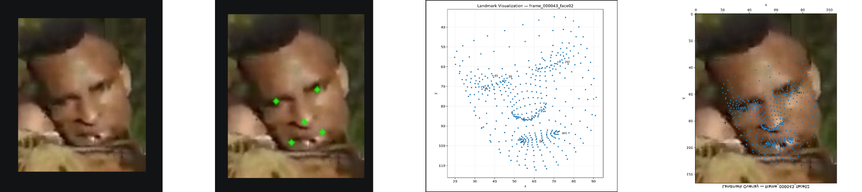
\includegraphics[width=0.85\textwidth]{figures/ringkasan-pipeline-wajah}
\caption[Ringkasan alur satu potongan wajah melalui pipeline]{Ringkasan alur satu potongan wajah melalui \textit{pipeline}: potongan wajah hasil deteksi, titik fitur geometris (empat titik hijau) yang dipakai untuk fitur jarak alis/bibir/mulut, visualisasi titik-fitur \textit{mesh} 468-titik MediaPipe, dan hasil tumpang-susun \textit{mesh} tersebut pada potongan wajah yang sama.}
\label{fig:ringkasan-pipeline}
\end{figure}

Gambar~\ref{fig:ringkasan-pipeline} memberi gambaran sekilas tentang apa yang dimaksud ``potongan wajah'' dan ``titik-fitur'' di seluruh bab ini, sebelum rinciannya dijelaskan per komponen pada \S\ref{sec:dataset-overview} dan \S\ref{sec:methodology-landmarks}.

\section{Dataset Lama dan Dua Populasi Evaluasi}
\label{sec:dataset-overview}

Seluruh eksperimen FER (EXP-005 sampai EXP-008, serta analisis ulang EXP-010 dan EXP-011) memakai potongan dari satu video sumber: film dokumenter pesta babi masyarakat Papua, resolusi 1920$\times$1080, berdurasi sekitar 96 menit, 144.084 \textit{frame} pada 25 fps.

\begin{figure}[htbp]
\centering
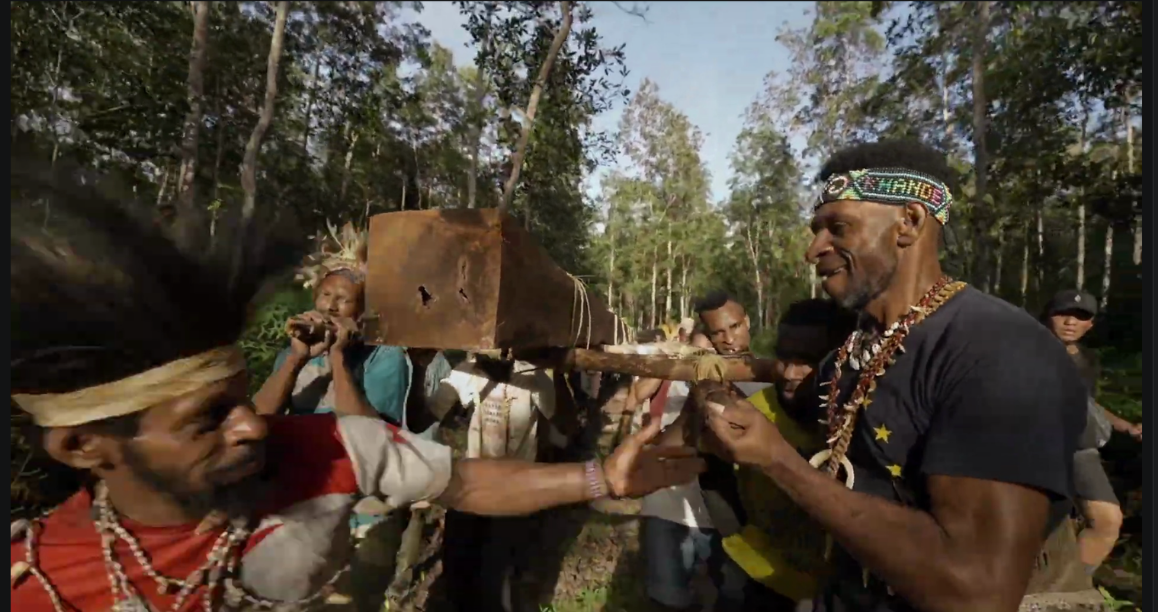
\includegraphics[width=0.7\textwidth]{figures/contoh-frame-sumber}
\caption[Contoh satu frame dari film sumber]{Contoh satu \textit{frame} dari film sumber, sebelum deteksi wajah dijalankan.}
\label{fig:contoh-frame-sumber}
\end{figure}

Gambar~\ref{fig:contoh-frame-sumber} menunjukkan satu \textit{frame} mentah seperti ini, sebelum tahap deteksi wajah (\S\ref{sec:arcface-config} di bawah, dan \S\ref{sec:clahe-config}) dijalankan terhadapnya. Satu kali jalan \textit{pipeline} berskala uji-coba (\textit{debug-scale}) terhadap 100 \textit{frame} yang diambil sampelnya menghasilkan 227 potongan wajah terdeteksi melalui paket \texttt{buffalo\_l} milik InsightFace (pendeteksi SCRFD, bantalan kotak pembatas 20\%). Setiap satu dari 227 potongan itu diperiksa secara manual oleh satu orang anotator dan diberi salah satu dari tujuh label: Netral (80), Ambigu (83), Senang (34), Sedih (12), Jijik (2), Takut (7), Terkejut (8), Marah (1). Tidak ada anotator kedua yang memeriksa label-label ini, dan proyek ini tidak memiliki statistik kesepakatan antar-anotator untuknya. Batasan ini berlaku untuk setiap hasil dalam bab ini dan bab berikutnya, dinyatakan sekali di sini.

Untuk setiap potongan, kelompok warna kulit dihitung langsung dari data piksel: kombinasi berbobot dari rata-rata, median, dan rata-rata wilayah tengah kanal-L ruang warna LAB (\texttt{src/landmark\_analyzer.py}, fungsi \texttt{\_compute\_skin\_tone}), diberi ambang batas menjadi beberapa kelompok (Gelap di bawah 100, Gelap-Sedang di bawah 150, dan seterusnya). Ini adalah statistik kecerahan, bukan pengukuran demografis, dan disebut sebagai ``proksi warna kulit'' di seluruh tesis ini agar perbedaan ini tetap terlihat dalam teks, tidak hanya di catatan kaki. Pada sampel 227 potongan, fungsi ini menghasilkan 159 potongan Gelap, 65 Gelap-Sedang, dan 3 Gelap-Terang, bukan populasi yang nyaris seragam seperti yang diasumsikan oleh deskripsi internal dataset ini sebelumnya. (Pembagian kira-kira 59\%/41\% yang pernah dilaporkan berasal dari 85 potongan yang memiliki fitur titik-fitur wajah, bukan dari seluruh 227 potongan; \texttt{research-audit/D8\_SKIN\_TONE\_DISCREPANCY\_INVESTIGATION.md}.)

\textbf{Dua populasi dipakai dalam eksperimen-eksperimen ini, dan keduanya tidak bisa dipertukarkan begitu saja.} EXP-005 dan EXP-006 mengevaluasi HSEmotion terhadap seluruh sampel 227 potongan dalam pelabelan tujuh-kelas aslinya. EXP-007 mengevaluasi baik HSEmotion maupun klasifier berbasis ArcFace pada subset turunan berjumlah 135 potongan, dibatasi menjadi lima kelas (Takut, Senang, Netral, Sedih, Terkejut). Subset 135 potongan inilah populasi utama untuk ketiga RQ: EXP-010 (RQ1, RQ3) dan EXP-011 (RQ2) menghitung kesenjangan antar-kelompok pada subset ini, sedangkan hasil pada 227 potongan dipakai hanya sebagai bukti pendukung. Subset 135 potongan ini bukan sampel yang dikumpulkan terpisah; subset ini adalah populasi 227 potongan yang disaring melalui tiga langkah pengecualian berturut-turut, masing-masing dengan penyebab yang konkret dan terdokumentasi:

\begin{enumerate}
  \item 83 potongan berlabel \texttt{Ambigu} dibuang, karena ``Ambigu'' bukan kelas ekspresi target dan klasifier tidak punya cara yang berprinsip untuk dinilai terhadapnya. $227 - 83 = 144$.
  \item 1 potongan \texttt{Marah} dan 2 potongan \texttt{Jijik} dibuang sebagai pengecualian kelas jarang, karena keduanya tidak punya cukup kejadian untuk mendukung metrik per-kelas yang dapat diandalkan pada ukuran sampel ini. $144 - 3 = 141$.
  \item 6 potongan lagi hilang akibat kegagalan deteksi ulang ArcFace: \textit{pipeline} ArcFace menjalankan ulang deteksi wajah pada setiap potongan yang sudah ada sebelum mengekstraksi \textit{embedding}-nya (\S\ref{sec:arcface-config}), dan 6 dari 141 potongan yang memenuhi syarat label gagal pada langkah deteksi ulang ini sehingga dikecualikan. $141 - 6 = 135$.
\end{enumerate}

Rangkaian ini dikuatkan oleh dua dokumen proyek yang independen, yaitu hitungan titik-periksa laporan evaluasi R6/R7 (227 $\to$ 178 berhasil dideteksi ulang $\to$ 144 memenuhi syarat label $\to$ 135 akhir) dan urutan penyaringan yang ditetapkan dalam dokumen rancangan eksperimen, dan penggabungan datanya sendiri berbasis identitas (dicocokkan berdasarkan nama berkas potongan wajah, diverifikasi secara terprogram), bukan berdasarkan posisi baris. Satu bukti konkret yang menguatkan hal ini: 18 kesalahan klasifikasi Netral-menjadi-Marah yang terhitung pada populasi penuh 227 potongan, jatuh persis, di dalam subset 135 potongan ketika hitungan yang sama diambil di sana. Hal ini tidak akan terjadi apabila subset 135 potongan adalah populasi yang diekstraksi ulang secara independen, bukan hasil penyaringan ketat dari populasi 227 potongan. Inilah sebabnya pula hipotesis internal sebelumnya, bahwa subset 135 potongan berasal dari ekstraksi ulang ``Papuan V2'' yang terpisah, sudah diselidiki dan dicabut (\texttt{RESEARCH\_DECISIONS.md}, Keputusan 3). Yang masih belum terverifikasi adalah identitas persis dari 6 potongan yang hilang pada langkah deteksi ulang; aturan dan aritmetikanya sudah mapan, daftar baris-per-barisnya belum.

\section{Komponen \textit{Pipeline}}

\subsection{Deteksi dan Pemotongan Wajah}

Deteksi memakai paket \texttt{buffalo\_l} milik InsightFace (pendeteksi SCRFD) pada resolusi 640$\times$640, inferensi CPU, dengan margin bantalan 20\% ditambahkan ke setiap kotak pembatas sebelum pemotongan. Tahap ini hanya menemukan dan memotong wajah; tidak melakukan klasifikasi atau ekstraksi fitur dalam bentuk apa pun.

\begin{figure}[htbp]
\centering
\begin{subfigure}[b]{0.3\textwidth}
\centering
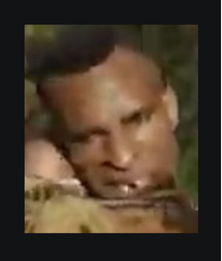
\includegraphics[width=\textwidth]{figures/contoh-potongan-wajah}
\caption{Potongan wajah hasil deteksi}
\end{subfigure}
\hfill
\begin{subfigure}[b]{0.3\textwidth}
\centering
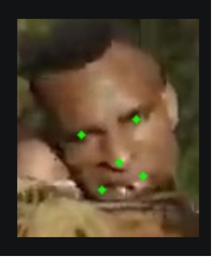
\includegraphics[width=\textwidth]{figures/contoh-fitur-geometris}
\caption{Empat titik fitur geometris}
\end{subfigure}
\hfill
\begin{subfigure}[b]{0.3\textwidth}
\centering
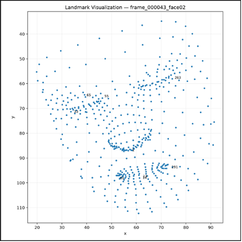
\includegraphics[width=\textwidth]{figures/contoh-visualisasi-titik-fitur}
\caption{Visualisasi \textit{mesh} 468-titik}
\end{subfigure}
\caption[Tiga tahap representasi untuk satu potongan wajah yang sama]{Tiga tahap representasi untuk satu potongan wajah yang sama: (a) hasil pemotongan langsung dari pendeteksi SCRFD, (b) empat titik fitur geometris MediaPipe (jarak alis, sudut bibir, bukaan mulut, jarak antar-mata), dan (c) \textit{mesh} 468-titik penuh milik MediaPipe yang dipakai untuk menurunkan titik-titik pada (b). Panel (b) dan (c) adalah fitur geometris dari \textit{pipeline} lama (lihat juga Bab~\ref{chap:literature-review}) dan bukan masukan bagi tiga eksperimen FER pada Bab~\ref{chap:results}; disertakan di sini semata untuk memperjelas apa yang dimaksud ``titik-fitur'' bagi pembaca yang tidak terbiasa dengan istilah \textit{computer vision}.}
\label{fig:tiga-tahap-wajah}
\end{figure}

\subsection{HSEmotion: Inferensi dengan Model Terlatih}

Berkas ekspor ONNX milik HSEmotion (\texttt{enet\_b0\_8\_best\_vgaf}) dijalankan persis seperti yang dipublikasikan: bobotnya tidak diubah di mana pun dalam proyek ini, dan keluaran \textit{softmax}-nya atas kosakata delapan-kelas yang sudah tetap (Marah, Jijik, Takut, Senang, Netral, Sedih, Terkejut, dan Merendahkan, \textit{Contempt}) diambil langsung sebagai prediksi. Kelas \textit{Contempt} tidak punya padanan pada label manusia; pada 227 potongan, HSEmotion tidak sekali pun memprediksi \textit{Contempt}, sehingga kelas ini tidak memengaruhi hasil apa pun dalam tesis ini. Ini adalah satu-satunya konfigurasi yang dipakai pada EXP-005 maupun EXP-006; kedua eksperimen hanya berbeda pada apakah CLAHE diterapkan pada potongan wajah sebelum tahap ini dijalankan.

\subsection{Konfigurasi CLAHE (RQ2)}
\label{sec:clahe-config}

Varian CLAHE pada EXP-006 berada di \texttt{notebooks/\allowbreak preprocessing\_experiment.ipynb} dan secara eksplisit bukan bagian dari \textit{pipeline} produksi (\texttt{src/\allowbreak fer\_dataset/\allowbreak pipeline/\allowbreak emotion\_classifier.py} tidak menerapkan praproses semacam ini). Transformasi ini hanya bekerja pada kanal-L ruang warna LAB, dengan batas klip yang menyesuaikan estimasi kecerahan berbobot tiap potongan, antara batas bawah 1,5 dan batas atas 3,5, pada rentang kecerahan masukan 60--220, diterapkan dengan kisi ubin (\textit{tile}) $8\times8$. Setiap potongan yang sudah disesuaikan dengan CLAHE kemudian diklasifikasi ulang dengan model HSEmotion beku yang sama seperti pada EXP-005, dan hasilnya dibandingkan terhadap prediksi pada potongan asli (tanpa modifikasi) dari eksperimen yang sama, pada 227 potongan yang sama, sehingga perbandingan sebelum/sesudah ini bersifat model-sama, sampel-sama, hanya satu varian praproses yang berubah. Ini adalah satu kali eksekusi saja, tanpa pengulangan, dan EXP-006 sendiri tidak menghitung selang kepercayaan maupun uji signifikansi. Selang kepercayaan dan uji McNemar untuk perbandingan ini kemudian dihitung pada subset 135 potongan oleh EXP-011, dari prediksi EXP-006 yang sudah tersimpan tanpa inferensi ulang (\S\ref{sec:fairness-methods}).

\subsection{\textit{Embedding} ArcFace dan Klasifier Regresi Logistik (RQ3)}
\label{sec:arcface-config}

\textit{Embedding} ArcFace dihasilkan dengan menjalankan ulang deteksi dan penyelarasan (\textit{alignment}) wajah pada setiap gambar potongan 227-potongan yang sudah ada (bukan pada \textit{frame} video asli), melalui submodel \texttt{buffalo\_l/w600k\_r50} milik InsightFace, menghasilkan vektor 512-dimensi yang sudah dinormalisasi-L2 untuk setiap potongan yang berhasil diselaraskan. Langkah deteksi ulang inilah sumber dari hitungan 178-dari-227 keberhasilan penyelarasan (\S\ref{sec:dataset-overview}), dan tempat terjadinya 6 dari pengecualian akhir populasi 135 potongan. Bobot ArcFace dibekukan sepenuhnya: ArcFace hanya menyumbang representasi yang tetap, tidak ada yang disesuaikan (\textit{fine-tuned}) pada data proyek ini.

Klasifier yang dilatih di atas \textit{embedding} ini adalah Regresi Logistik multinomial, teregularisasi-L2, berbobot-kelas, dipilih dan divalidasi dengan validasi silang \texttt{StratifiedGroupKFold} lima-lipatan (\textit{seed} 42), dengan potongan-potongan dikelompokkan ke dalam blok temporal 3-\textit{frame} sebelum dibagi ke lipatan. Pengelompokan ini ada karena tidak tersedia kolom identitas subjek pada dataset ini (\S\ref{sec:leakage}); pengelompokan berdasarkan kedekatan waktu adalah pengganti heuristik, bukan jaminan terverifikasi bahwa individu yang sama tidak pernah muncul di dua lipatan berbeda. Tidak ada partisi uji terpisah yang disisihkan di luar lipatan validasi silang. Angka akurasi dan pola kesalahan yang dilaporkan pada Bab~\ref{chap:results} \S\ref{sec:rq3-results} adalah estimasi hasil validasi silang atas seluruh populasi 135 potongan, bukan dari satu pembagian latih/uji tunggal.

\subsection{Metrik Evaluasi}
\label{sec:metrics}

Tiga prosedur statistik dipakai, masing-masing untuk tujuan tertentu, dan tidak satu pun bisa saling menggantikan. Uji McNemar \citep{mcnemar1947note} (EXP-007, RQ3) membandingkan pasangan hasil benar/salah dari dua klasifier pada 135 potongan yang sama, sebuah pemakaian yang direkomendasikan \citet{dietterich1998approximate} untuk membandingkan dua klasifier yang masing-masing hanya dijalankan sekali karena tingkat galat tipe I-nya rendah, dan menguji apakah ketidaksepakatan di antara keduanya simetris; uji ini menjawab ``apakah ada perbedaan yang terdeteksi,'' bukan ``apakah kedua klasifier setara''. Perbedaan ini terus ditegaskan pada Bab~\ref{chap:results} mengingat sampel ini hanya punya 46 pasangan yang tidak sepakat. \textit{Bootstrap} yang sadar-kelompok (2.000 pengambilan ulang sampel, mengambil ulang berdasarkan 16 kelompok temporal, bukan per potongan individu) menghasilkan selang kepercayaan 95\% untuk akurasi tiap klasifier, menghormati ketidak-bebasan data yang sama yang melandasi validasi silang berkelompok di atas. Uji eksak Fisher (EXP-005/007) menguji apakah kelompok proksi warna kulit dan kebenaran klasifikasi berasosiasi secara statistik pada sampel ini; hasil yang signifikan dari uji ini adalah bukti adanya asosiasi pada sampel khusus dan tidak acak ini, bukan bukti bahwa variabel proksi tersebut menyebabkan hasil klasifikasi.

\subsection{Evaluasi Kesenjangan Antar-Kelompok (EXP-010 dan EXP-011)}
\label{sec:fairness-methods}

Ketiga RQ dijawab pada populasi yang sama, yaitu subset 135 potongan lima-kelas (\S\ref{sec:dataset-overview}). Kedua eksperimen ini adalah analisis ulang atas prediksi yang sudah tersimpan: tidak ada model yang dilatih atau dijalankan ulang, dan tidak ada label, dataset, atau berkas prediksi yang diubah. EXP-010 membaca prediksi HSEmotion dan ArcFace + LR dari EXP-007; EXP-011 membaca prediksi HSEmotion pada potongan asli dan potongan CLAHE dari EXP-006. Keduanya dapat direproduksi dengan \texttt{tools/\allowbreak analyze\_fairness\_135.py} dan \texttt{tools/\allowbreak analyze\_clahe\_fairness\_135.py}, dan keluarannya terbukti identik pada setiap jalan.

\textbf{Pengelompokan.} Pada EXP-007/008, kelompok kecerahan hanya tersedia untuk 78 dari 135 potongan, karena diambil dari berkas fitur titik-fitur wajah yang hanya mencakup 85 potongan. EXP-010 menjalankan fungsi yang sama (\texttt{\_compute\_skin\_tone}) pada potongan \textbf{asli} untuk seluruh 135 potongan. Hasilnya mereproduksi ke-78 kelompok yang sudah ada tanpa perbedaan (78/78) dan menghasilkan Gelap 89 dan Gelap-Sedang 46; tidak ada potongan Gelap-Terang atau Terang. Hasil dilaporkan dengan pengelompokan 135 potongan sebagai analisis utama dan pengelompokan 78 potongan sebagai pemeriksaan stabilitas. Pada EXP-011, kelompok yang sama dipakai untuk kedua kondisi, sehingga CLAHE tidak memindahkan potongan antar-kelompok; kolom kelompok pada berkas EXP-006 juga cocok dengan kelompok ini pada 135/135 potongan.

\textbf{Pemetaan kelas.} Label HSEmotion dipetakan ke penamaan tesis ini (\textit{Anger}$\to$Marah, \textit{Happiness}$\to$Senang, \textit{Sadness}$\to$Sedih), sama dengan pemetaan pada \texttt{tools/\allowbreak evaluate\_arcface\_vs\_hsemotion.py}. Prediksi Marah dihitung sebagai salah karena berada di luar lima kelas evaluasi. Berkas EXP-006 menyimpan label yang sudah dipetakan, sedangkan EXP-007 menyimpan nama asli keluaran model; perbandingan literal hanya cocok pada 88 dari 135 potongan, tetapi setelah pemetaan yang sama, prediksi potongan asli EXP-006 identik dengan prediksi HSEmotion EXP-007 pada 135/135 potongan. Perbedaan ini hanya soal penamaan, bukan perbedaan data.

\textbf{Metrik.}
\begin{itemize}
  \item \textit{Akurasi}: proporsi potongan yang prediksinya sama dengan kebenaran lapangan.
  \item \textit{F1 makro}: rata-rata F1 tiap kelas. Untuk keseluruhan, dirata-ratakan atas lima kelas; untuk tiap kelompok, atas kelas yang ada pada kelompok tersebut.
  \item \textit{Kesenjangan}: akurasi Gelap dikurangi akurasi Gelap-Sedang.
  \item \textit{Akurasi kelompok terburuk}: akurasi terendah di antara kedua kelompok, ukuran yang lazim dipakai untuk menilai kinerja model pada kelompok yang paling dirugikan \citep{sagawa2020dro}.
  \item \textit{Recall} per kelas di dalam kelompok, hanya untuk Netral dan Senang, karena kelas lain terlalu kecil pada kelompok Gelap-Sedang.
\end{itemize}

\textbf{Perbandingan.} EXP-010 membandingkan HSEmotion dan ArcFace + LR, termasuk selisih kesenjangan kedua model (kesenjangan HSEmotion dikurangi kesenjangan ArcFace + LR). EXP-011 membandingkan HSEmotion pada potongan asli dan potongan CLAHE, dengan perubahan dihitung sebagai CLAHE dikurangi asli untuk akurasi, akurasi per kelompok, dan kesenjangan.

\textbf{Uji dan selang kepercayaan.} Uji McNemar eksak (uji binomial atas pasangan yang tidak sepakat) dijalankan untuk seluruh potongan dan untuk tiap kelompok. Selang kepercayaan 95\% dihitung dengan \textit{bootstrap} berkelompok yang sama dengan EXP-007: 16 blok waktu (indeks \textit{frame} dibagi 3) diambil ulang dengan pengembalian, 2.000 kali, dan batas 2,5 serta 97,5 persentil diambil sebagai selang. Gagasan mengambil ulang blok observasi yang berurutan, bukan observasi tunggal, untuk data yang saling bergantung berasal dari \textit{block bootstrap} \citep{kunsch1989jackknife}. Varian yang dipakai di sini lebih sederhana: blok tetap yang tidak tumpang-tindih dan panjangnya ditentukan secara heuristik (3 \textit{frame}), bukan blok bergerak dengan panjang yang dipilih secara teoretis. Pengelompokan ini hanya mengatasi ketergantungan antar-potongan dari \textit{frame} yang berdekatan; pengelompokan ini tidak mengendalikan kemunculan ulang orang yang sama di bagian film yang berjauhan (\S\ref{sec:leakage}). Setiap selang memakai pembangkit acak baru dengan \textit{seed} 42. Untuk ukuran yang membandingkan dua kelompok atau dua kondisi (kesenjangan, selisih kesenjangan, perubahan akurasi), kedua sisi dihitung pada sampel \textit{bootstrap} yang sama, sehingga perbandingannya berpasangan. F1 makro dilaporkan tanpa selang kepercayaan.

\textbf{Batasan analisis.} Uji McNemar per kelompok dan seluruh perbandingan antar-kelompok tidak dikoreksi untuk perbandingan berganda dan diperlakukan sebagai eksploratif. Kedua eksperimen bersifat retrospektif: prediksi yang dianalisis sudah ada sebelum RQ dirumuskan. HSEmotion dipakai apa adanya, sedangkan prediksi ArcFace + LR berasal dari validasi silang berkelompok (\S\ref{sec:arcface-config}), sehingga kedua model tidak dievaluasi dengan protokol yang sama. Kelompok Gelap-Sedang hanya berisi 46 potongan, sehingga daya uji per kelompok rendah; hasil yang tidak signifikan tidak dibaca sebagai bukti tidak adanya pengaruh. \textit{Bootstrap} blok waktu hanya sebagian mengatasi kemunculan orang yang sama pada beberapa potongan (\S\ref{sec:leakage}).

\section{Titik-Fitur Wajah: Jalur Pendukung yang Masih Berjalan}
\label{sec:methodology-landmarks}

\subsection{Papuan V2}
\label{sec:papuan-v2}

Papuan V2 adalah ekstraksi kedua yang independen dari film sumber yang sama, dengan jalan pengambilan sampel yang berbeda (\texttt{max\_frames=250}, 2,0 fps), menghasilkan 645 potongan wajah dengan cabang olahan-CLAHE paralel, dan tidak berbagi satu pun potongan dengan populasi 227/135 potongan yang dipakai untuk RQ1 sampai RQ3. Subset uji coba berjumlah 150 gambar diambil untuk uji coba anotasi, dan alur kerja anotasi manusia disiapkan memakai dua instansi server Label Studio yang terisolasi: satu untuk anotator utama yang mengerjakan seluruh 150 gambar uji coba, satu lagi untuk anotator kedua yang mengerjakan subset tumpang-tindih 75 gambar yang dimaksudkan untuk mendukung pengukuran kesepakatan antar-anotator begitu keduanya selesai. Tidak satu pun yang selesai: antrean tugas anotator tumpang-tindih menunjukkan nol dari 75 tugas terkumpul pada status terakhir yang tercatat, dan klaim penyelesaian penuh oleh anotator utama belum diverifikasi ulang secara independen terhadap berkas ekspor mentahnya untuk revisi ini (\texttt{research-audit/DATA\_DISCREPANCIES.md} D-1). Secara terpisah, HSEmotion dan klasifier berbasis ArcFace sama-sama dijalankan terhadap 150 gambar uji coba ini, menghasilkan prediksi tanpa ada label manusia yang tersedia untuk dibandingkan.

\subsection{Dari Label Emosi ke Titik-Fitur, dan Posisi Uji Coba Ini Sekarang}

Di tengah perjalanan proyek ini, target anotasi untuk uji coba Papuan V2 diubah, atas arahan dosen pembimbing, dari label emosi menjadi titik-fitur wajah. Perubahan ini terbatas pada target anotasi uji coba ini saja, bukan perubahan arah penelitian tesis secara keseluruhan, yang tetap FER (\texttt{RESEARCH\_DECISIONS.md}, Keputusan 2). Konvensi yang dipakai adalah 68 titik mengikuti ibug-300W, dengan koordinat awal dibuat otomatis oleh submodel \texttt{landmark\_3d\_68} milik InsightFace dan dimuat ke instansi CVAT lokal untuk diperiksa. Uji coba 24-gambar diisi dengan cara ini, dan skema penamaan titik milik proyek ini sendiri ditulis ulang dari pengenal generik (\texttt{pt0} hingga \texttt{pt67}) menjadi nama anatomis yang deskriptif, perubahan yang sudah diverifikasi tidak menggeser koordinat sama sekali.

\begin{figure}[htbp]
\centering
\begin{subfigure}[b]{0.32\textwidth}
\centering
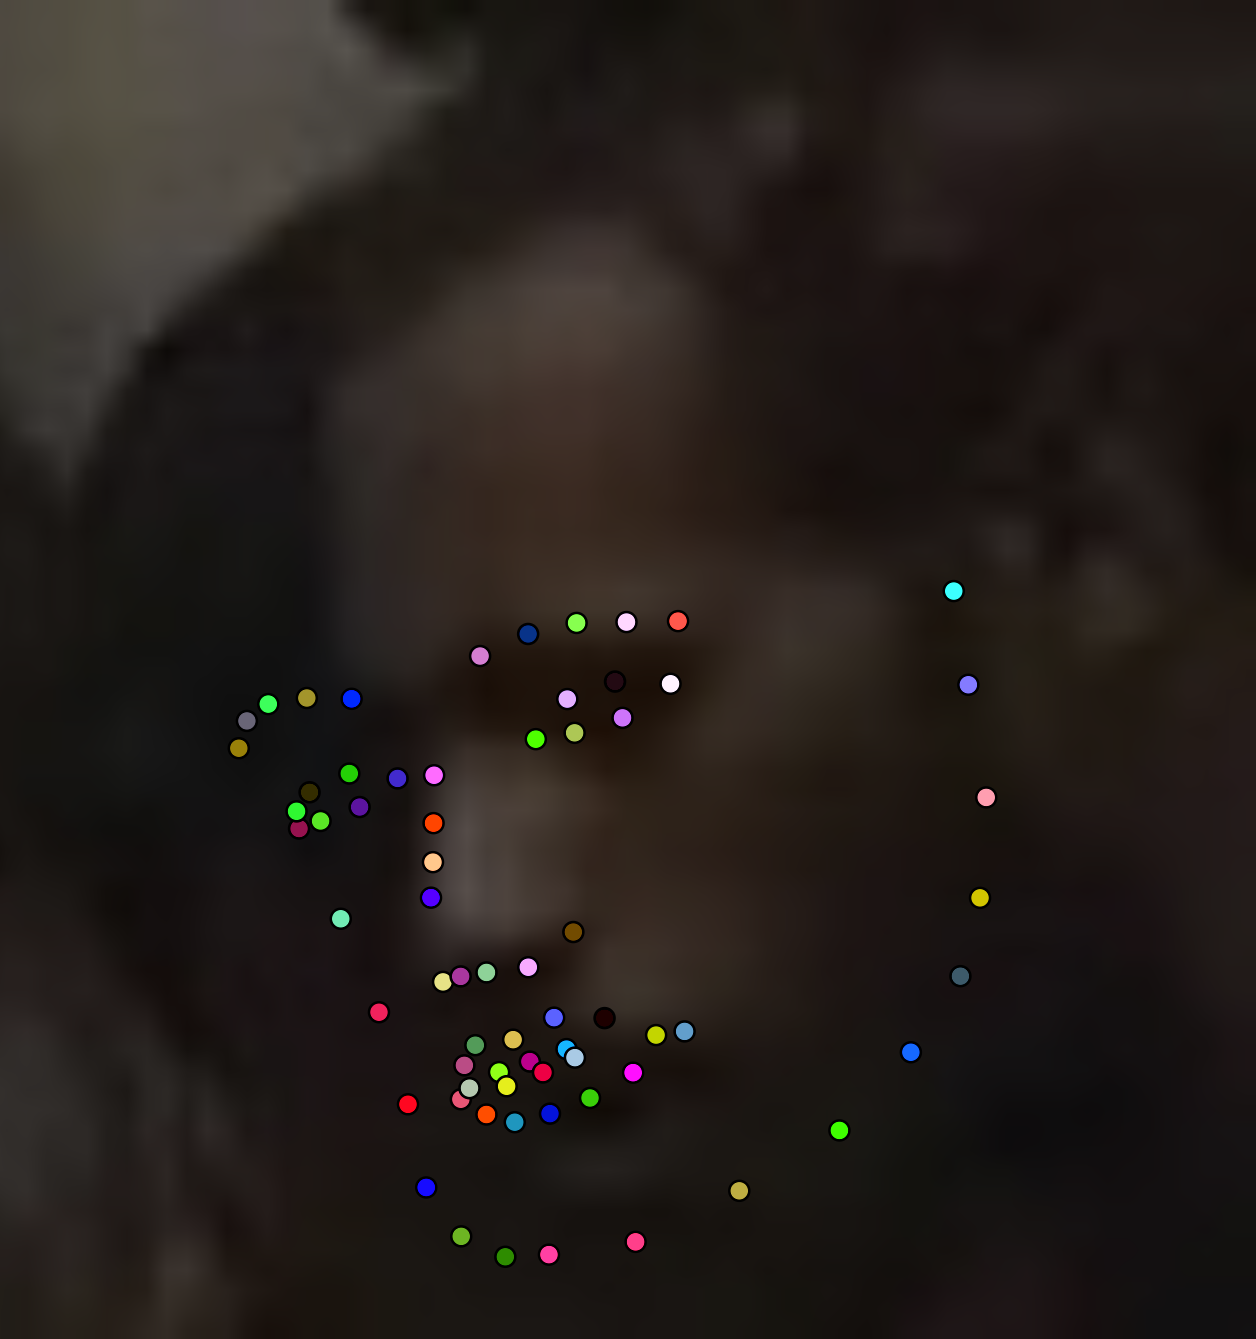
\includegraphics[width=\textwidth]{figures/contoh-anotasi-cvat-68-titik}
\caption{68 titik usulan otomatis}
\end{subfigure}
\hfill
\begin{subfigure}[b]{0.3\textwidth}
\centering
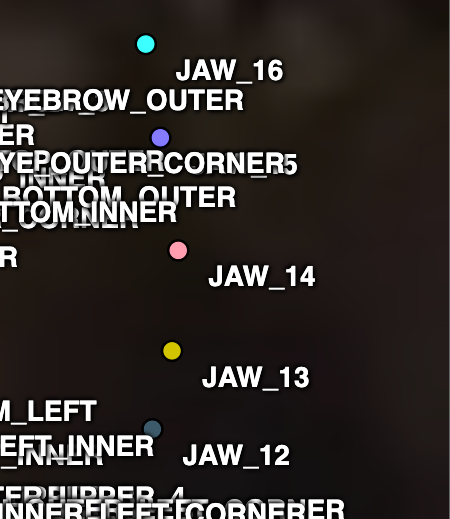
\includegraphics[width=\textwidth]{figures/contoh-label-anatomis-kanvas-cvat}
\caption{Label anatomis pada kanvas}
\end{subfigure}
\hfill
\begin{subfigure}[b]{0.3\textwidth}
\centering
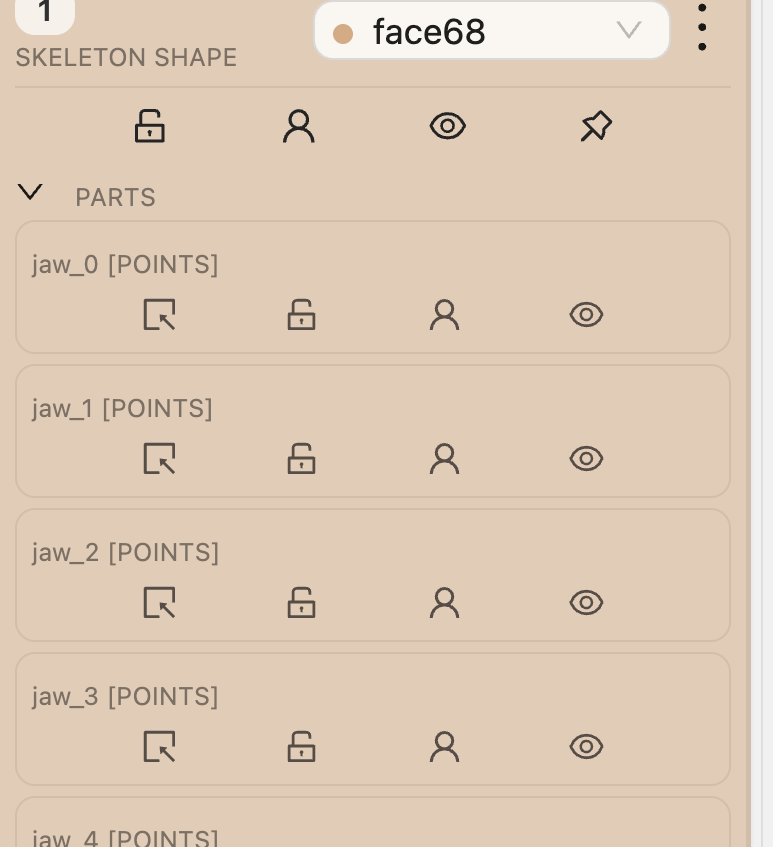
\includegraphics[width=\textwidth]{figures/contoh-skema-penamaan-cvat}
\caption{Panel \textit{Parts} CVAT}
\end{subfigure}
\caption[Tangkapan layar uji coba CVAT 24-gambar]{Tangkapan layar instansi CVAT lokal pada uji coba 24-gambar, potongan wajah \texttt{frame\_000009\_face04}: (a) 68 titik usulan otomatis dari submodel \texttt{landmark\_3d\_68} milik InsightFace, sebelum pemeriksaan manusia; (b) label anatomis (mis.\ \texttt{JAW\_16}, \texttt{JAW\_14}) tampil langsung pada kanvas, menggantikan pengenal generik \texttt{pt0}--\texttt{pt67}; (c) panel \textit{Parts} CVAT yang sama menunjukkan skema penamaan (\texttt{jaw\_0}, \texttt{jaw\_1}, dst.) untuk \textit{skeleton shape} \texttt{face68}. Titik-titik ini adalah usulan otomatis yang belum diperiksa; tidak ada koreksi manusia yang terekam pada tangkapan layar ini.}
\label{fig:cvat-pilot-68-titik}
\end{figure}

\textbf{Pembaruan sejak revisi sebelumnya: pemeriksaan manusia dan uji coba pelatihan awal sudah dilakukan, tetapi hasilnya tetap bersifat awal (\textit{preliminary}) dan tidak menunjukkan hasil yang meyakinkan.} Pemeriksaan manusia sudah diselesaikan untuk 64 gambar Original: 24 gambar dari uji coba awal (CVAT Task 1) dan 40 gambar tambahan dari uji coba kalibrasi (CVAT Task 3), keduanya diperiksa oleh satu peninjau yang sama -- belum ada peninjau kedua atau protokol kesepakatan antar-peninjau untuk titik-fitur, keterbatasan yang sejajar dengan yang sudah dinyatakan untuk populasi 227/135 potongan pada \S\ref{sec:dataset-overview}. Dari 64 gambar yang sudah diperiksa ini, satu pembagian \textit{train}/\textit{validation}/\textit{test} (45/11/8 gambar) dibuat dengan benih tetap (\texttt{seed=400}), dikelompokkan berdasarkan kedekatan nomor \textit{frame} karena tidak ada kolom identitas subjek yang tersedia di repositori ini -- keterbatasan yang sama persis dengan \S\ref{sec:leakage}, bukan jaminan bebas-kebocoran yang terverifikasi.

Dua model dasar dilatih dan dievaluasi pada pembagian ini, keduanya pada potongan Original saja: (1) model rerata-bentuk (\textit{mean-shape}) yang sepenuhnya mengabaikan isi piksel gambar, sebagai batas bawah pembanding; dan (2) regresi Ridge (\texttt{sklearn.linear\_model.Ridge}) pada fitur piksel \textit{grayscale} $32\times32$ yang diubah ukurannya dan diratakan (1.024 fitur), meregresi ke-68 titik sekaligus. \textbf{Regresi Ridge belum menunjukkan perbaikan yang berarti dibandingkan model rerata-bentuk pada 8 gambar uji yang disisihkan} -- Gambar~\ref{fig:ridge-vs-meanshape} menunjukkan galat piksel yang hampir identik di antara keduanya pada hampir setiap gambar uji, bukan hanya pada rata-ratanya. Model Ridge yang sama (tidak dilatih ulang) juga dievaluasi pada versi CLAHE dari gambar uji yang sama, memakai koordinat target yang tidak diubah -- sah dilakukan karena CLAHE pada proyek ini sudah diverifikasi secara terpisah tidak mengubah geometri gambar (lihat Gambar~\ref{fig:titik-clahe-original}). Hasilnya juga hampir identik dengan versi Original, yang konsisten dengan model ini belum benar-benar memanfaatkan isi piksel secara berarti -- \textbf{ini bukan bukti bahwa model titik-fitur yang sungguh-sungguh belajar dari piksel akan menunjukkan ketahanan yang sama terhadap CLAHE}, hanya bahwa model saat ini belum cukup sensitif terhadap piksel untuk diuji pada pertanyaan itu.

\begin{figure}[htbp]
\centering
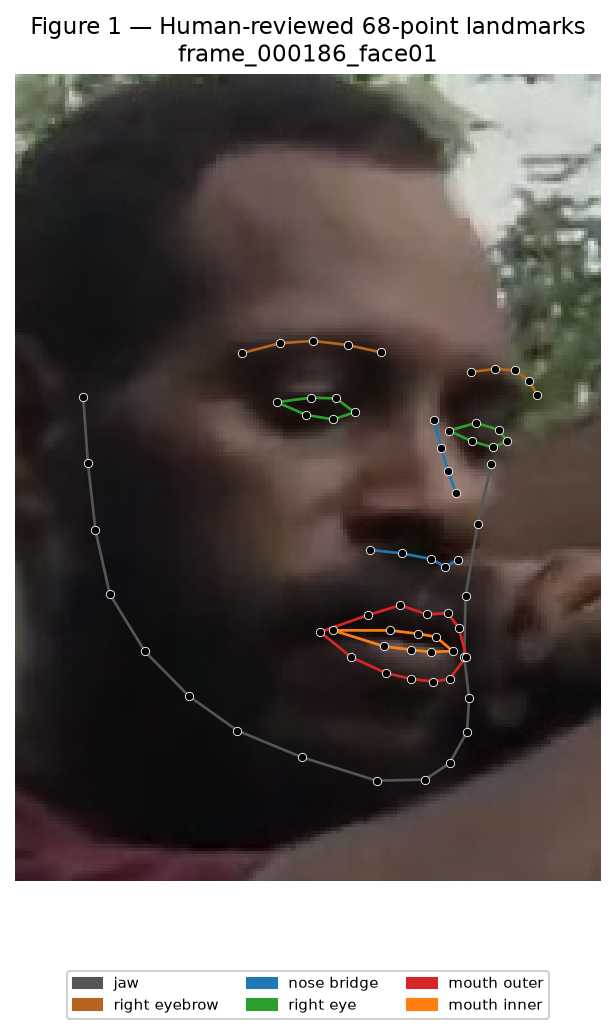
\includegraphics[width=0.7\textwidth]{figures/contoh-titik-fitur-diperiksa-manusia}
\caption[Contoh titik-fitur yang sudah diperiksa manusia]{Satu gambar dengan 68 titik-fitur yang sudah diperiksa manusia, diberi warna menurut wilayah wajah (rahang, alis, mata, hidung, mulut).}
\label{fig:titik-fitur-diperiksa}
\end{figure}

\begin{figure}[htbp]
\centering
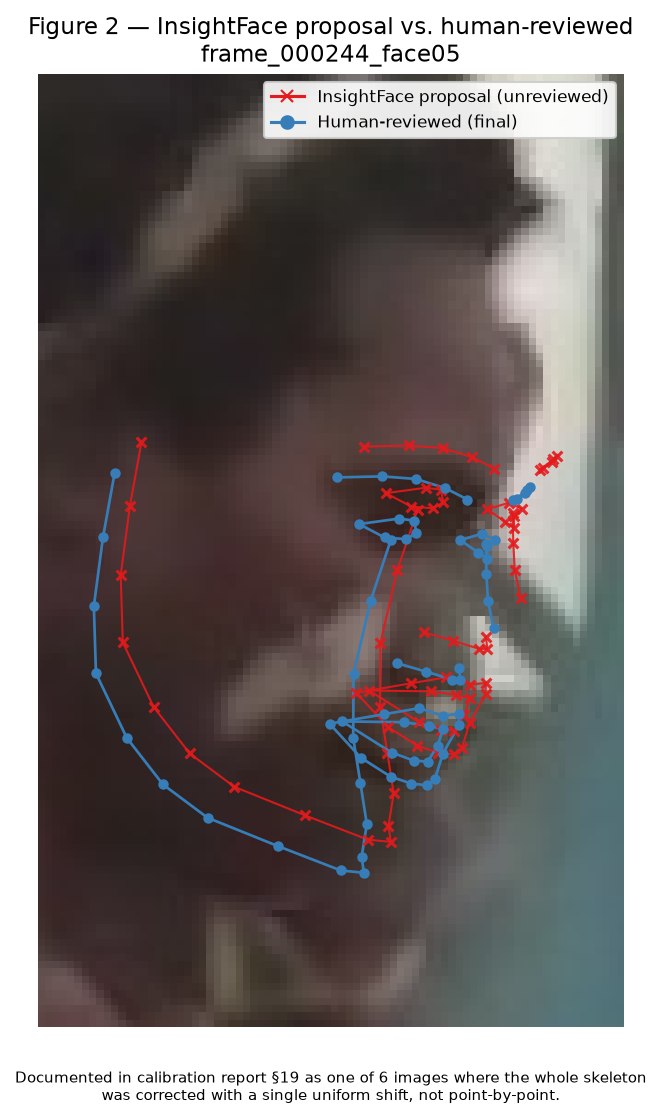
\includegraphics[width=0.6\textwidth]{figures/perbandingan-usulan-vs-diperiksa}
\caption[Usulan otomatis dibandingkan hasil pemeriksaan manusia]{Usulan otomatis InsightFace (merah, tanda ×) dibandingkan hasil akhir setelah pemeriksaan manusia (biru, titik) pada gambar yang sama -- satu dari beberapa gambar yang dikoreksi dengan menggeser seluruh \textit{skeleton} sekaligus, bukan titik demi titik, sebagaimana didokumentasikan dalam catatan uji coba kalibrasi proyek ini.}
\label{fig:usulan-vs-diperiksa}
\end{figure}

\begin{figure}[htbp]
\centering
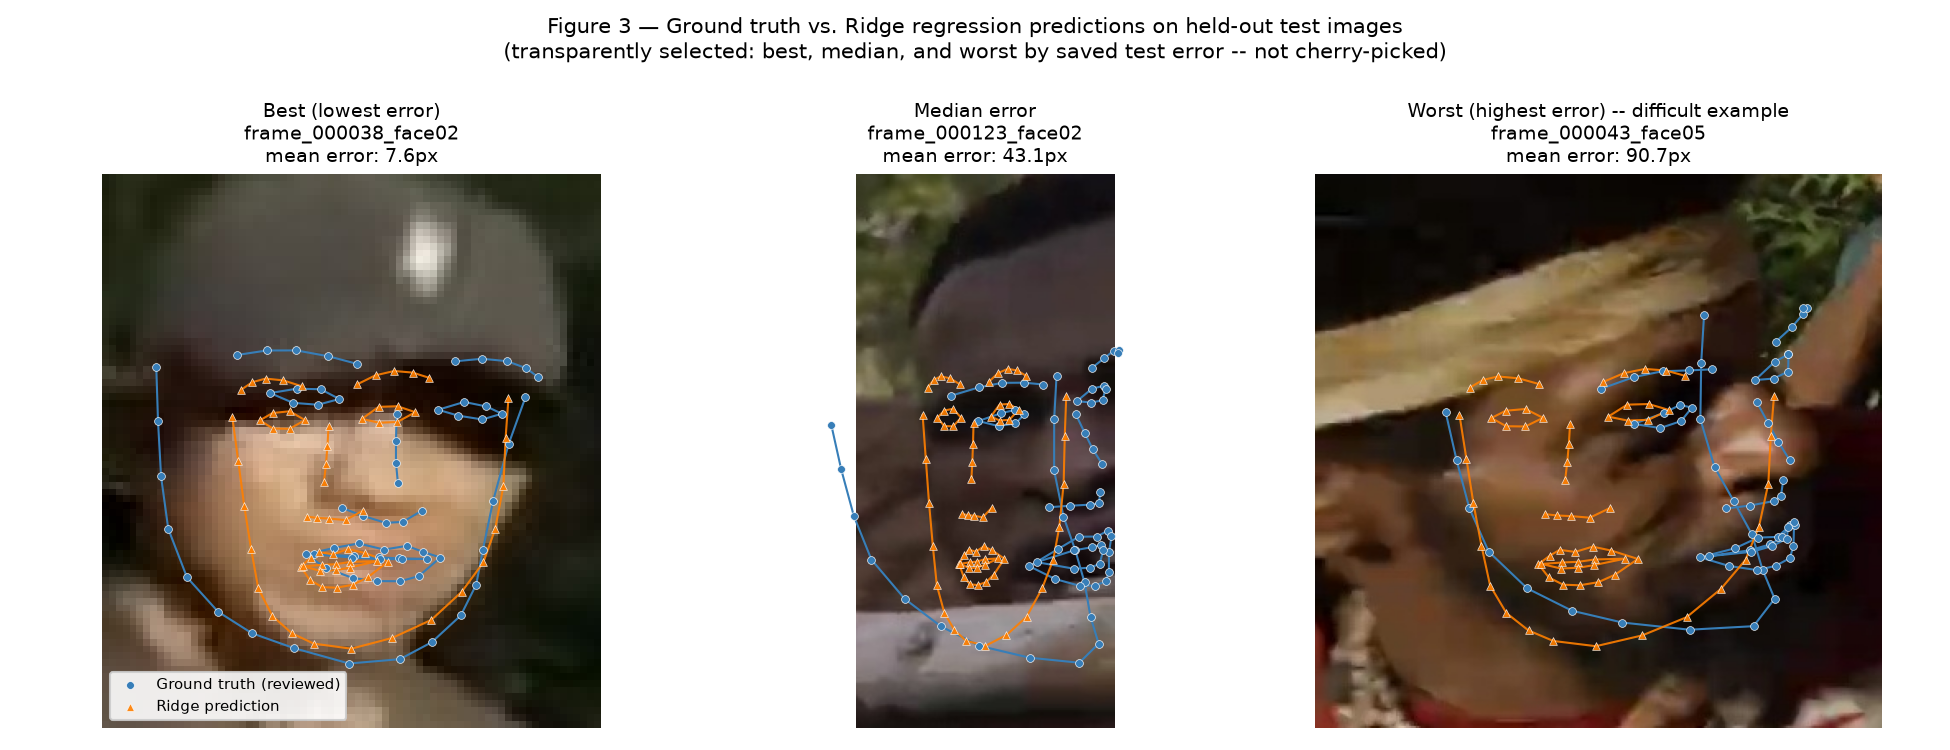
\includegraphics[width=0.85\textwidth]{figures/kebenaran-vs-prediksi-ridge}
\caption[Kebenaran lapangan dibandingkan prediksi Ridge pada gambar uji]{Kebenaran lapangan (biru) dibandingkan prediksi regresi Ridge (oranye) pada tiga gambar uji yang dipilih secara transparan -- gambar dengan galat terendah, median, dan tertinggi dari seluruh 8 gambar uji -- bukan dipilih karena hasilnya terlihat baik.}
\label{fig:ridge-vs-meanshape}
\end{figure}

\begin{figure}[htbp]
\centering
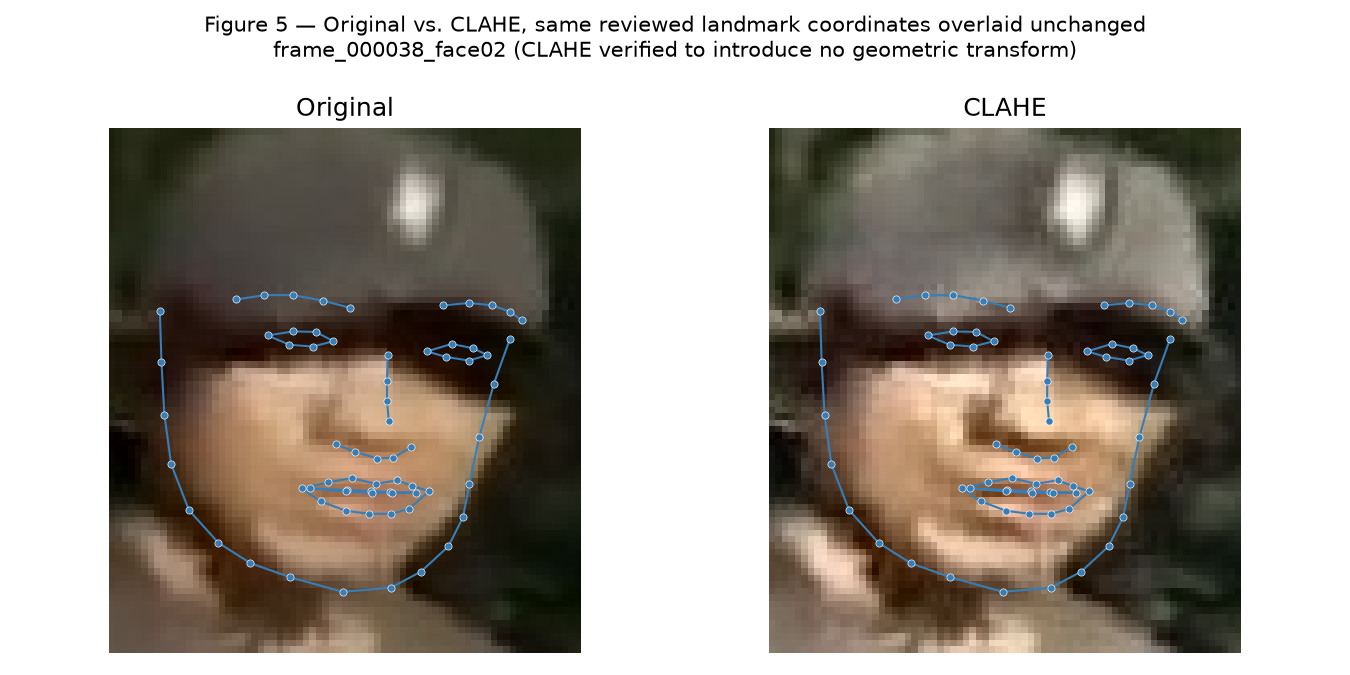
\includegraphics[width=0.75\textwidth]{figures/titik-fitur-original-vs-clahe}
\caption[Titik-fitur yang sama pada gambar Original dan CLAHE]{Koordinat titik-fitur hasil pemeriksaan manusia yang identik, ditumpangkan tanpa perubahan pada versi Original (kiri) dan CLAHE (kanan) dari potongan wajah yang sama -- mengonfirmasi secara visual bahwa transformasi CLAHE pada proyek ini tidak mengubah geometri gambar.}
\label{fig:titik-clahe-original}
\end{figure}

Yang masih belum ada, dinyatakan secara eksplisit agar tidak tersirat lebih dari yang sebenarnya: belum ada peninjau kedua atau statistik kesepakatan antar-peninjau untuk titik-fitur; cakupan pemeriksaan baru 64 dari 645 gambar yang tersedia ($<$10\%); belum ada bukti bahwa pendekatan berbasis piksel apa pun benar-benar mengungguli \textit{mean-shape} pada data sebesar ini; dan tidak ada klaim ketahanan umum terhadap CLAHE, soal keadilan (\textit{fairness}), maupun generalisasi di luar sampel kecil ini. Rincian lengkap metodologi pelatihan, pembagian data, dan hasil per-gambar didokumentasikan di luar naskah tesis ini pada \texttt{docs/reports/PAPUAN\_V2\_ANNOTATION\_CALIBRATION\_PLAN.md} (artefak repositori, bukan lampiran tesis formal). Masing-masing dari keterbatasan ini adalah kerja lanjutan, didaftar beserta bukti yang diperlukan untuk menyatakannya selesai, pada Bab~\ref{chap:conclusion} \S\ref{sec:future-work}. Tidak ada apa pun dalam tesis ini yang mengklaim, menyiratkan, atau bergantung pada uji coba ini sudah terbukti berguna atau dapat diandalkan sebagai model titik-fitur, dan tidak ada satu pun hasil pada Bab~\ref{chap:results} yang bersyarat pada hal itu.

\section{Identitas Subjek, Kebocoran Data, dan Batas Kemampuan Pengelompokan}
\label{sec:leakage}

Tidak ada kolom pada kedua dataset yang menandai potongan mana saja yang menunjukkan orang yang sama. Pengelompokan temporal 3-\textit{frame} yang dipakai untuk validasi silang EXP-007 (\S\ref{sec:arcface-config}) berasumsi bahwa \textit{frame} yang berdekatan waktu lebih mungkin menunjukkan subjek yang sama dalam pose yang nyaris identik dibanding \textit{frame} yang berjauhan. Ini adalah heuristik yang masuk akal untuk rekaman dokumenter satu kamera, tetapi bukan jaminan yang terverifikasi. Seorang subjek yang keluar lalu muncul kembali ke adegan di bagian film yang lebih belakangan akan terpecah ke kelompok yang berbeda oleh skema ini, dan tidak ada apa pun dalam \textit{pipeline} saat ini yang akan menangkap kejadian tersebut. Hal ini membatasi seberapa kuat estimasi validasi silang pada \S\ref{sec:rq3-results} bisa dibaca sebagai bebas-dari-pengaruh-subjek-yang-sama, dan hal ini dinyatakan ulang pada bagian Bab~\ref{chap:results} di mana hal ini relevan dengan angka tertentu, bukan hanya di sini.

% Sumber: reports/audit_summary_metrics.csv, reports/audit_per_skin_tone_accuracy.csv,
% reports/preprocessing_experiment_summary.csv (melalui docs/EXPERIMENT.md EXP-006),
% reports/arcface_evaluation/{comparison_metrics,statistical_tests,skin_tone_analysis}.csv,
% reports/arcface_error_analysis/neutral_error_analysis.csv, docs/EXPERIMENT.md,
% docs/EXP-007_ARCFACE_EVALUATION.md, research-audit/DATA_DISCREPANCIES.md (D-8).
\chapter{Hasil dan Pembahasan}
\label{chap:results}

Bab ini menjawab RQ1, RQ2, dan RQ3 secara berurutan. Setiap bagian tetap berada dalam populasinya sendiri: 227 potongan, tujuh-kelas, untuk RQ1 dan RQ2; subset 135 potongan, lima-kelas, untuk RQ3. Tidak satu pun menggabungkan angka dari satu populasi dengan angka dari populasi lain tanpa menyatakannya secara eksplisit.

\section{RQ1: Karakteristik Kesalahan Garis Dasar HSEmotion pada Sampel 227 Potongan}
\label{sec:rq1-results}

Keluaran HSEmotion (model terlatih, dipakai apa adanya) pada 227 potongan tanpa modifikasi mencapai akurasi keseluruhan 22,47\% terhadap kebenaran lapangan satu-anotator, dengan 17,62\% dari seluruh 227 prediksi berupa panggilan ``Marah'' yang salah (Marah diprediksi padahal label aslinya bukan itu). Memecah tingkat salah-Marah ini berdasarkan label asli menunjukkan di mana ia terkonsentrasi: 18 dari 76 potongan berlabel-asli Netral (23,7\%) diprediksi Marah, yang merupakan pola kesalahan tunggal terbesar yang bisa diidentifikasi pada sampel ini, lebih besar, dalam hitungan mutlak, dibanding pasangan kebingungan (\textit{confusion}) lain mana pun.

Dua kelompok proksi warna kulit yang dikarakterisasi pada sampel ini menunjukkan akurasi yang mencolok bedanya: 44,0\% untuk potongan Gelap berbanding 14,3\% untuk potongan Gelap-Sedang, selisih 29,7 poin persentase (dihitung sebagai selisih maksimum-dikurangi-minimum sederhana antara dua kelompok ini, bukan ukuran efek yang dinormalisasi atau metrik keadilan tingkat-populasi). Uji eksak Fisher pada data yang sama menghasilkan rasio odds 5,88 ($p = 0,0027$), yang mendukung bahwa kelompok ini dan hasil klasifikasi berasosiasi secara statistik pada sampel ini. Hasil ini tidak mendukung pembacaan sebab-akibat. Kedua kelompok ini adalah statistik kecerahan yang dihitung per potongan, bukan ukuran demografis yang tervalidasi (Bab~\ref{chap:methodology} \S\ref{sec:dataset-overview}), dan tidak ada apa pun dalam rancangan sampel ini (satu film sumber, satu kamera, satu tata pencahayaan, tanpa pengacakan dalam bentuk apa pun) yang memisahkan variabel proksi ini dari faktor-faktor yang berkorelasi, seperti adegan mana yang kebetulan menjadi sumber potongan tiap kelompok. Asosiasi sekuat ini layak dilaporkan secara presisi; asosiasi ini, dengan sendirinya, bukanlah penjelasan.

Ada satu catatan yang lebih pantas ditulis di sini daripada di catatan kaki. \textit{Notebook} ablasi-CLAHE milik proyek ini sendiri (EXP-006) memuat perhitungan per-kelompok-warna-kulit kedua yang dihitung secara independen, dan angka ``sebelum''-nya, yaitu pada potongan tanpa modifikasi, untuk dua kelompok yang sama adalah 27,7\% (Gelap) dan 10,8\% (Gelap-Sedang), bukan 44,0\% dan 14,3\%, meskipun kedua \textit{notebook} melaporkan akurasi keseluruhan yang identik, 22,47\%, untuk kondisi yang seharusnya sama. Perbedaan ini dicatat lengkap pada \texttt{research-audit/DATA\_DISCREPANCIES.md} (butir D-8) dan belum terselesaikan pada revisi ini. Logika pengelompokan per-baris pada kedua \textit{notebook} tersebut belum diperiksa langsung, karena berkas CSV mentah dari keduanya tidak tersedia untuk diturunkan ulang dalam repositori ini. Tesis ini melaporkan angka EXP-005 di atas sebagai nilai acuan, karena EXP-005 adalah audit warna kulit yang memang dirancang khusus untuk itu, sedangkan perhitungan pada EXP-006 adalah keluaran sampingan dari ablasi yang tujuannya berbeda; tesis ini tidak mengklaim bahwa kedua \textit{notebook} ini saling mengonfirmasi, karena pada perhitungan spesifik ini keduanya jelas-jelas tidak sama.

Apa yang terbukti dan apa yang tidak terbukti, dinyatakan secara gamblang: terbukti bahwa model ini, pada sampel ini, berkinerja jauh di bawah yang biasa dilaporkan pada benchmark-nya sendiri, dengan satu kesalahan yang spesifik dan cukup besar, terkonsentrasi pada satu kelas ekspresi dan satu arah kebingungan. Tidak terbukti mengapa, baik untuk akurasi agregat yang rendah, maupun untuk selisih proksi warna kulit, dan tidak terbukti apa pun tentang perilaku model ini terhadap wajah masyarakat Papua sebagai sebuah populasi, karena 227 potongan dari satu film bukanlah sampel yang dirancang untuk mendukung generalisasi semacam itu.

\section{RQ2: Pengaruh Konfigurasi CLAHE yang Diuji}
\label{sec:rq2-results}

Menerapkan varian CLAHE adaptif yang dijelaskan pada Bab~\ref{chap:methodology} \S\ref{sec:clahe-config} pada 227 potongan yang sama, lalu menjalankan ulang model HSEmotion beku yang sama, mengubah akurasi keseluruhan dari 22,47\% menjadi 19,82\% dan tingkat salah-Marah dari 17,62\% menjadi 18,06\%. Kedua angka ini bergerak ke arah yang berlawanan dengan dugaan hipotesis eksperimen itu sendiri: judul \textit{notebook} sumbernya sendiri menyatakan bahwa uji ini dimaksudkan untuk melihat apakah CLAHE akan mengurangi prediksi salah-Marah dan memperbaiki kesetaraan antar-proksi warna kulit, dan pada jalan uji ini CLAHE tidak melakukan keduanya.

\begin{figure}[htbp]
\centering
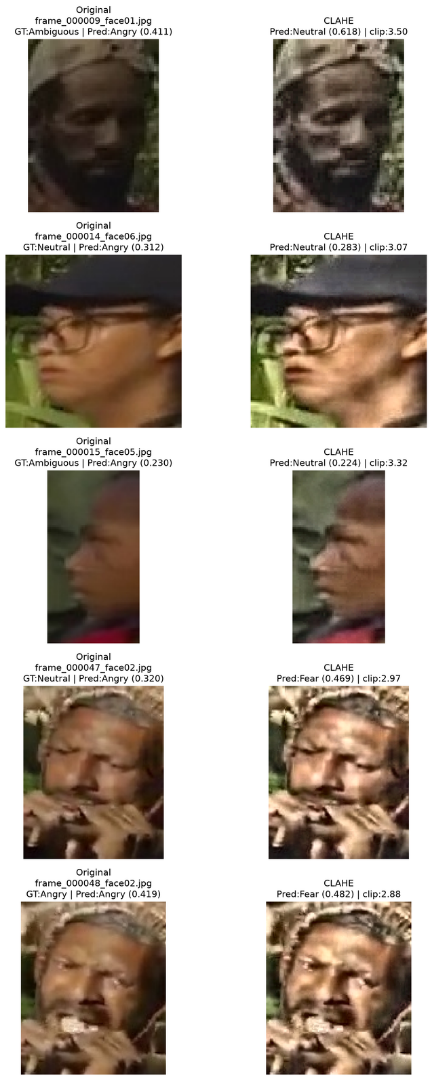
\includegraphics[width=0.35\textwidth]{figures/perbandingan-clahe-sebelum-sesudah}
\caption[Contoh kualitatif potongan wajah sebelum dan sesudah CLAHE]{Contoh kualitatif perbandingan potongan wajah asli (kiri) dan hasil olahan CLAHE (kanan), dengan label kebenaran lapangan (GT), prediksi HSEmotion, dan nilai batas klip (\textit{clip limit}) adaptif yang dipakai untuk tiap potongan. Batas klip terlihat bervariasi antar-potongan (2,88 hingga 3,50), sesuai mekanisme yang dijelaskan pada \S\ref{sec:clahe-config}: batas klip menyesuaikan estimasi kecerahan tiap potongan secara individual, bukan nilai tetap untuk seluruh sampel. Gambar ini untuk ilustrasi mekanisme saja; angka akurasi agregat 22,47\%$\to$19,82\% di atas dihitung atas seluruh 227 potongan, bukan hanya lima contoh yang ditampilkan di sini.}
\label{fig:clahe-contoh}
\end{figure}

Gambar~\ref{fig:clahe-contoh} menunjukkan efek visual CLAHE pada beberapa contoh potongan: kontras memang berubah, dan pada beberapa contoh prediksi model ikut berubah (misalnya dari ``Angry'' menjadi ``Neutral'' atau ``Fear''), tetapi perubahan tersebut tidak konsisten ke satu arah, sejalan dengan angka agregat di atas yang menunjukkan hasil bersihnya justru sedikit memburuk, bukan membaik.

Ini adalah satu kali eksekusi tanpa pengulangan, dan tanpa selang kepercayaan atau uji signifikansi yang dihitung untuk kedua selisih tersebut (Bab~\ref{chap:methodology} \S\ref{sec:clahe-config}). Penurunan akurasi 2,65 poin persentase dan kenaikan salah-Marah 0,44 poin, yang teramati satu kali saja, tidak membuktikan bahwa konfigurasi CLAHE tertentu ini merugikan dengan keyakinan statistik apa pun, apalagi bahwa CLAHE sebagai teknik praproses pada umumnya merugikan. Rentang batas klip yang berbeda, pemetaan kecerahan yang berbeda, atau sekadar variasi acak dari pengulangan sampel, semuanya bisa saja, pada prinsipnya, menggeser hasil ini. Yang didukung oleh pengamatan ini, pada lingkup yang benar-benar diukur, lebih sempit dan tetap layak dinyatakan secara langsung: untuk konfigurasi CLAHE adaptif ini, model ini, dan sampel ini, langkah praproses tersebut tidak memberikan perbaikan yang menjadi tujuan pengujiannya, dan seorang peneliti yang harus memilih antara memakai konfigurasi ini atau tidak, tidak akan menemukan bukti di sini yang membenarkan pemakaiannya.

\section{RQ3: HSEmotion Berbanding Regresi Logistik Berbasis ArcFace pada Subset 135 Potongan}
\label{sec:rq3-results}

\textbf{Perbandingan ini dijalankan sebelum versi apa pun dari pertanyaan penelitian tesis ini ditulis.} Hasil ini dilaporkan di sini sebagai analisis retrospektif atas bukti yang sudah ada sebelumnya, menjawab RQ3 belakangan, bukan sebagai uji konfirmatif yang memang dirancang di muka untuk menghasilkan RQ3 (Bab~\ref{chap:introduction} \S\ref{sec:rq}). Perbedaan ini memengaruhi seberapa besar bobot yang semestinya diberikan pada hasil di bawah ini: hasil yang diperoleh dengan cara ini tetaplah bukti yang sah, tetapi bobot konfirmatifnya lebih kecil dibanding perbandingan yang dirancang di muka khusus untuk menjawab pertanyaan tersebut.

\begin{table}[h]
\centering
\caption[Perbandingan HSEmotion dan ArcFace+Regresi Logistik]{HSEmotion berbanding ArcFace+Regresi Logistik, subset 135 potongan, lima kelas. Sumber: berkas hasil evaluasi ArcFace (metrik perbandingan dan uji statistik) pada proyek ini.}
\label{tab:rq3-comparison}
\begin{tabular}{lrr}
\toprule
Metrik & HSEmotion & ArcFace + LR \\
\midrule
Akurasi & 36,30\% & 40,74\% \\
Presisi makro & 0,590 & 0,280 \\
\textit{Recall} makro & 0,206 & 0,293 \\
F1 makro & 0,249 & 0,272 \\
SK 95\% \textit{bootstrap} (akurasi, sadar-kelompok) & [0,269, 0,467] & [0,338, 0,481] \\
\bottomrule
\end{tabular}
\end{table}

Akurasi titik ArcFace+LR (40,74\%) secara angka lebih tinggi dari HSEmotion (36,30\%) pada subset ini, tetapi uji McNemar pada 46 prediksi yang tidak sepakat (20 berpihak pada ArcFace+LR, 26 berpihak pada HSEmotion) menghasilkan $p = 0,4614$: tidak ada perbedaan yang terdeteksi pada tingkat signifikansi yang lazim. Inilah seluruh klaim dari hasil ini: uji McNemar yang tidak signifikan pada ukuran sampel ini berarti perbedaannya tidak terdeteksi, bukan berarti kedua klasifier setara. Dengan hanya 46 pasangan yang tidak sepakat sebagai bahan uji, perbedaan nyata yang ukurannya sedang-sedang saja bisa dengan mudah luput terdeteksi di sini; tesis ini tidak membaca hasil nihil ini sebagai temuan bahwa kedua pendekatan berkinerja sama.

Angka presisi/\textit{recall}/F1 makro tidak menunjukkan satu klasifier yang unggul di segala aspek: presisi makro HSEmotion lebih tinggi, sementara \textit{recall} dan F1 makro ArcFace+LR lebih tinggi. Ini sejalan dengan dugaan bahwa kedua klasifier membuat jenis kesalahan yang berbeda, bukan satu klasifier yang sekadar membuat lebih sedikit kesalahan dibanding yang lain. Perbedaan ini terlihat langsung pada bagaimana masing-masing model menangani kelas Netral, kelas terbesar dalam subset ini (76 dari 135 potongan): HSEmotion salah mengklasifikasi 34 dari 76 potongan Netral, dan kesalahan tersebut terkonsentrasi kuat ke satu arah, 18 di antaranya berlabel Marah. ArcFace+LR salah mengklasifikasi lebih banyak potongan Netral (43 dari 76) tetapi menyebarkannya ke empat kelas lain (Senang 15, Sedih 14, Takut 8, Terkejut 6) tanpa satu target kebingungan yang dominan. Klasifier yang membuat lebih banyak kesalahan total tetapi menghindari satu pola kegagalan yang timpang tidak serta-merta lebih buruk untuk semua keperluan, dan tesis ini tidak mengurutkan kedua pendekatan hanya berdasarkan akurasi semata.

Pada perhitungan proksi warna kulit dalam subset 135 potongan yang sama ini, kedua klasifier mencapai akurasi 45,65\% pada kelompok Gelap ($n=46$); pada kelompok Gelap-Sedang ($n=32$), ArcFace+LR mencapai 31,25\% berbanding 12,50\% milik HSEmotion, selisih antar-kelompok proksi yang lebih kecil untuk ArcFace+LR (14,4 poin) dibanding HSEmotion (33,2 poin) pada subset ini. Ini adalah satu pengamatan tunggal yang belum direplikasi pada satu kelompok berisi 32 potongan, bukan perbaikan keadilan yang sudah terbukti, dan tesis ini tidak memakainya sebagai bukti perbaikan keadilan. Hasil ini dilaporkan karena memang bagian dari apa yang ditunjukkan data, dengan bobot yang persis sebesar itu saja.

\section{Papuan V2: Status, Bukan Hasil}
\label{sec:rq-papuanv2-status}

Belum ada temuan kuantitatif dari jalur Papuan V2 yang layak masuk bab hasil, karena memang belum ada. Ekstraksi berskala uji-coba 645 potongan sudah selesai; uji coba anotasi label emosi belum (antrean anotator tumpang-tindih menunjukkan nol dari 75 tugas selesai pada status terakhir yang tercatat, dan klaim penyelesaian anotator utama belum diverifikasi ulang secara independen, \texttt{research-audit/DATA\_DISCREPANCIES.md} D-1); uji coba titik-fitur CVAT 24-gambar baru berisi usulan otomatis dan belum diperiksa manusia. Tidak satu pun dari RQ1 sampai RQ3 memakai jalur ini sebagai bukti, dan bagian ini ada semata agar pembaca tidak perlu menyimpulkan sendiri ketiadaannya dari keheningan. % TODO: isi dengan tabel hasil, berstruktur seperti Tabel~\ref{tab:rq3-comparison}, hanya setelah uji coba CVAT diperiksa dan dataset yang dihasilkan dievaluasi pada partisi uji yang disisihkan, bukan sebelum itu.

\section{Sintesis}

RQ1 dan RQ2 menjelaskan populasi 227 potongan yang sama di bawah dua kondisi praproses; RQ3 menjelaskan subset 135 potongan dari populasi yang sama di bawah dua klasifier. Jika dibaca bersama: akurasi HSEmotion pada sampel ini rendah dibanding kinerja yang biasa dilaporkan pada benchmark-nya, disertai selisih akurasi proksi warna kulit yang spesifik, besar, dan berasosiasi secara statistik (tidak terbukti sebab-akibat), serta pola kesalahan Netral-menjadi-Marah yang dominan dan tetap sama baik diukur pada 227 maupun 135 potongan; satu konfigurasi CLAHE yang diuji tidak membantu, dalam satu kali jalan uji yang tidak terkontrol; dan perbandingan retrospektif terhadap alternatif berbasis ArcFace tidak menemukan perbedaan akurasi keseluruhan yang signifikan secara statistik, disertai sebaran kesalahan yang secara kualitatif berbeda dan tidak setimpang untuk klasifier alternatif tersebut. Tidak satu pun dari ini berlaku umum melampaui satu film sumber sampel ini, dan tidak satu pun dari ini menjadi bukti tentang jalur Papuan V2, yang tetap merupakan pekerjaan terpisah dan belum selesai.

% Sumber: disusun dari Bab 4 tesis ini (EXP-005 sampai EXP-011); tidak ada klaim baru yang diperkenalkan di sini.
\chapter{Kesimpulan}
\label{chap:conclusion}

\section{Jawaban atas Pertanyaan Penelitian}

\textbf{RQ1.} Pada subset 135 potongan, akurasi HSEmotion adalah 0,483 pada kelompok Gelap dan 0,130 pada kelompok Gelap-Sedang, dengan kesenjangan 0,353 (SK 95\% [0,182; 0,540]). Kesenjangan ini tetap terlihat di dalam kelas Netral dan Senang, dan sebagian besar berasal dari potongan Netral Gelap-Sedang yang diprediksi Marah (12 dari 21). Arah yang sama teramati pada sampel 227 potongan. Ini adalah asosiasi pada satu sampel, bukan bukti bahwa warna kulit menjadi penyebabnya.

\textbf{RQ2.} Konfigurasi CLAHE adaptif yang diuji mengubah kesenjangan dari 0,353 menjadi 0,330 (perubahan $-$0,023; SK 95\% [$-$0,136; 0,073]). Pengaruhnya terhadap kesenjangan tidak dapat disimpulkan dari data ini; hasil ini tidak membuktikan bahwa CLAHE tidak berpengaruh. Kesenjangan tetap besar dengan maupun tanpa CLAHE, dan laju prediksi Marah pada Gelap-Sedang tidak berubah (0,478).

\textbf{RQ3.} ArcFace + Regresi Logistik memiliki kesenjangan yang lebih kecil (0,123; SK 95\% [$-$0,038; 0,282]) karena akurasinya pada Gelap-Sedang lebih tinggi (0,326 berbanding 0,130), sementara akurasi Gelap-nya tidak lebih baik. Selisih kesenjangan kedua model tidak memuat nol pada pengelompokan 135 potongan (0,229; SK 95\% [0,054; 0,442]) tetapi memuat nol pada pengelompokan 78 potongan (0,188; SK 95\% [$-$0,083; 0,477]), sehingga pengurangan kesenjangan ini bersifat indikatif, belum terbukti. Akurasi keseluruhan kedua model tidak berbeda secara signifikan (McNemar $p = 0,4614$), dan perbandingan ini bersifat retrospektif.

\section{Ringkasan}
\label{sec:summary}

Tesis ini mengevaluasi kesenjangan kinerja dua pendekatan pengenalan ekspresi wajah antara dua kelompok kecerahan kulit pada potongan wajah dari satu film dokumenter. Kesenjangan HSEmotion terukur dengan jelas pada sampel ini; satu konfigurasi praproses kontras tidak menghasilkan perubahan yang dapat disimpulkan; dan satu klasifier alternatif menunjukkan kesenjangan yang lebih kecil dengan bukti yang masih indikatif. Kedua kelompok sama-sama gelap, sehingga tesis ini tidak menjawab pertanyaan tentang kinerja pada kulit terang dibanding kulit gelap. Hasil ini tidak berlaku umum di luar sampel yang dievaluasi.

\section{Kontribusi}

Kontribusi tesis ini adalah: (1) evaluasi kesenjangan antar-kelompok kecerahan yang dapat direproduksi dari artefak tersimpan (EXP-010 dan EXP-011), lengkap dengan selang kepercayaan \textit{bootstrap} berkelompok; (2) dokumentasi bahwa pola kesalahan Netral$\to$Marah HSEmotion terkonsentrasi pada kelompok Gelap-Sedang dan menjelaskan sebagian besar kesenjangannya pada sampel ini; dan (3) pelaporan yang hati-hati atas dua intervensi sederhana, praproses dan penggantian klasifier, yang membedakan hasil yang tidak dapat disimpulkan dan hasil yang masih indikatif dari hasil yang sudah terbukti.

\section{Keterbatasan}

Keterbatasan dirinci pada Bab~\ref{chap:results} \S\ref{sec:results-limitations}. Yang paling membatasi klaim adalah: kelompok kecerahan sebagai proksi yang bercampur dengan pencahayaan dan hanya mencakup dua kelompok gelap; kelompok Gelap-Sedang yang kecil (46 potongan); satu film sumber dan satu anotator tanpa ukuran kesepakatan; ketiadaan identitas subjek; sifat retrospektif RQ3; dan dasar persetujuan serta asal-usul rekaman sumber yang belum terdokumentasi.

\section{Kerja Lanjutan}
\label{sec:future-work}

\begin{itemize}
  \item \textbf{Representasi kelompok.} Menambah potongan Gelap-Sedang serta kelompok yang lebih terang, dengan protokol perekaman dan persetujuan yang jelas, agar kesenjangan dapat diukur lebih presisi dan perbandingan kulit terang dan gelap menjadi mungkin.
  \item \textbf{Kualitas label.} Melibatkan anotator kedua dan melaporkan kesepakatan antar-anotator, termasuk menyelesaikan 75 potongan tumpang-tindih Papuan V2.
  \item \textbf{Validitas proksi.} Memeriksa secara manual sebagian kelompok kecerahan untuk menilai seberapa jauh kelompok tersebut dipengaruhi pencahayaan.
  \item \textbf{Pembagian data sadar-identitas.} Membangun identitas subjek atau jejak wajah agar partisi latih dan uji tidak berbagi orang yang sama.
  \item \textbf{Uji yang dirancang di muka.} Menguji pendekatan untuk memperkecil kesenjangan, misalnya klasifier berbobot kelompok, dengan kriteria keberhasilan yang ditetapkan sebelum evaluasi.
  \item \textbf{Privasi dan etika.} Menyelesaikan dasar persetujuan penggunaan rekaman, dan hanya memublikasikan hasil agregat serta ilustrasi wajah yang sudah dianonimkan.
  \item \textbf{Titik-fitur wajah.} Jalur titik-fitur tetap pekerjaan pendukung: 64 gambar sudah diperiksa manusia, tetapi belum ada model titik-fitur yang terbukti lebih baik daripada \textit{mean-shape} (\S\ref{sec:methodology-landmarks}), dan belum ada eksperimen terkontrol yang menghubungkan titik-fitur dengan kinerja klasifikasi emosi atau kesenjangannya.
\end{itemize}


% =============================================================
% bibliography.tex — Daftar Pustaka only
% =============================================================
% Juknis p.12-13: author-year style. The actual entries live in
% references.bib, not here -- edit that file to add/correct a
% citation (see README.md "Adding Chapters, Figures, Tables, and
% References" for the verification requirement before adding one).
% No Lampiran (appendix) section exists in this revision -- see
% FORMAT_COMPLIANCE.md "Appendices" for the rationale; if one is
% added later, it belongs in its own appendix.tex, not here.
% =============================================================

\bibliographystyle{\itbBibliographyStyle}
\bibliography{references}


\end{document}

